%!TEX encoding = UTF-8 Unicode

\documentclass[a4paper,11pt]{extarticle}
% L'option 'openany' permet de démarrer un chapitre sur une page paire

%-----------------------------------------------------------------------------------------------------------------------*
%                                                                                                                       *
%   R É G L A G E S    « F R A N Ç A I S »                                                                              *
%                                                                                                                       *
%-----------------------------------------------------------------------------------------------------------------------*

%--- Paquetage pour le codage des sources en UTF-8
\usepackage[utf8]{inputenc}

%--- Latex demande ce paquetage pour mieux afficher le caractère "°" et \textquotesingle "'"
\usepackage{textcomp}

%--- Ce paquetage permet d'effectuer certaines césures, et ainsi d'éviter les messages "Overfull \hbox"
\usepackage[T1]{fontenc}

\usepackage{lmodern}

%--- Paquetage pour imposer les réglages français
%\usepackage[frenchb]{babel}

%------------------------------------------------------------------------------------------------
%   C H O I X    D E    L A    P O L I C E
%------------------------------------------------------------------------------------------------

\usepackage[scaled=0.9, default]{sourcecodepro}
%\usepackage{fouriernc}
\usepackage[default]{sourcesanspro}

\usepackage[dvipsnames]{xcolor}

\usepackage{graphicx}

%-----------------------------------------------------------------------------------------------------------------------*
%                                                                                                                       *
%   M I S E    E N    P A G E                                                                                           *
%                                                                                                                       *
%-----------------------------------------------------------------------------------------------------------------------*

% Voir "Une courte introduction à Latex2e", § 6.4

%--- Marge gauche : 2,54 cm ; le paramètre \hoffset contient cette valeur, moins 1 pouce
%    \hoffset = 2,54 cm - 2,54 cm = 0 cm
\setlength{\hoffset}{0.cm}

%--- Marges supplémentaires, différenciées pour les pages gauches et droites ; ici, aucune.
\setlength{\oddsidemargin }{0 cm}
\setlength{\evensidemargin}{0 cm}

%--- Largeur du texte
%    \textwidth = 210 mm - 25.4 mm - 25.4 mm = 15,4 cm
\setlength{\textwidth}{15.92 cm}

%--- Marge haute : 2,54 cm ; le paramètre \voffset contient cette valeur, moins 1 pouce
%    \voffset = 2,54 cm - 2,54 cm = 0 cm
\setlength{\voffset}{0 cm}

%--- Distance entre la marge haute et l'en-tête : 0 cm
\setlength{\topmargin}{0 cm}

%--- Hauteur de l'en-tête de chaque page : 1 cm
\setlength{\headheight}{1 cm}

%--- Distance entre l'en-tête de chaque page et le corps : 0,5 cm
\setlength{\headsep}{0.5 cm}

%--- Hauteur du corps
%    \textheight = 29,7 cm - 2,54 cm - 2,8 cm - 1,5 cm = 22,6 cm
\setlength{\textheight}{22.86 cm}

%-----------------------------------------------------------------------------------------------------------------------*
%                                                                                                                       *
%   E X T E N S I O N S    P O U R    L ' É C R I T U R E    D E S     F O R M U L E S    M A T H É M A T I Q U E S     *
%                                                                                                                       *
%-----------------------------------------------------------------------------------------------------------------------*

%--- Extensions pour l'écriture des formules mathématiques
\usepackage{amsmath}
\usepackage{amssymb}
\usepackage{amsfonts}

%--- Paquetage "IEEEtrantools"
% Pour créer des tableaux d'équations, bien alignées
% Voir courte-intro-latex.pdf, page §3.5.2 page 83
\usepackage[retainorgcmds]{IEEEtrantools}

%-----------------------------------------------------------------------------------------------------------------------*

\usepackage{mdframed}

%-----------------------------------------------------------------------------------------------------------------------*
%                                                                                                                       *
%   P A Q U E T A G E    « L I S T I N G S »                                                                            *
%                                                                                                                       *
%-----------------------------------------------------------------------------------------------------------------------*

 %%%%%%%%%%%%%%%%%%%%%%%%%%%%%%%%%%%%%%%%%%%%%%%%%%%%%%%%%%%%%%%%%%%%%%%%%%%%%%%% 
%%% ~ Arduino Language - Arduino IDE Colors ~                                  %%%
%%%                                                                            %%%
%%% Kyle Rocha-Brownell | 10/2/2017 | No Licence                               %%%
%%% -------------------------------------------------------------------------- %%%
%%%                                                                            %%%
%%% Place this file in your working directory (next to the latex file you're   %%%
%%% working on).  To add it to your project, place:                            %%%
%%%     %%%%%%%%%%%%%%%%%%%%%%%%%%%%%%%%%%%%%%%%%%%%%%%%%%%%%%%%%%%%%%%%%%%%%%%%%%%%%%%% 
%%% ~ Arduino Language - Arduino IDE Colors ~                                  %%%
%%%                                                                            %%%
%%% Kyle Rocha-Brownell | 10/2/2017 | No Licence                               %%%
%%% -------------------------------------------------------------------------- %%%
%%%                                                                            %%%
%%% Place this file in your working directory (next to the latex file you're   %%%
%%% working on).  To add it to your project, place:                            %%%
%%%     %%%%%%%%%%%%%%%%%%%%%%%%%%%%%%%%%%%%%%%%%%%%%%%%%%%%%%%%%%%%%%%%%%%%%%%%%%%%%%%% 
%%% ~ Arduino Language - Arduino IDE Colors ~                                  %%%
%%%                                                                            %%%
%%% Kyle Rocha-Brownell | 10/2/2017 | No Licence                               %%%
%%% -------------------------------------------------------------------------- %%%
%%%                                                                            %%%
%%% Place this file in your working directory (next to the latex file you're   %%%
%%% working on).  To add it to your project, place:                            %%%
%%%    \input{arduinoLanguage.tex}                                             %%%
%%% somewhere before \begin{document} in your latex file.                      %%%
%%%                                                                            %%%
%%% In your document, place your arduino code between:                         %%%
%%%   \begin{lstlisting}[language=Arduino]                                     %%%
%%% and:                                                                       %%%
%%%   \end{lstlisting}                                                         %%%
%%%                                                                            %%%
%%% Or create your own style to add non-built-in functions and variables.      %%%
%%%                                                                            %%%
 %%%%%%%%%%%%%%%%%%%%%%%%%%%%%%%%%%%%%%%%%%%%%%%%%%%%%%%%%%%%%%%%%%%%%%%%%%%%%%%% 

\usepackage{color}
\usepackage{listings}    
\usepackage{courier}

%%% Define Custom IDE Colors %%%
\definecolor{arduinoGreen}    {rgb} {0.17, 0.43, 0.01}
\definecolor{arduinoGrey}     {rgb} {0.47, 0.47, 0.33}
\definecolor{arduinoOrange}   {rgb} {0.8 , 0.4 , 0   }
\definecolor{arduinoBlue}     {rgb} {0.01, 0.61, 0.98}
\definecolor{arduinoDarkBlue} {rgb} {0.0 , 0.2 , 0.5 }

%%% Define Arduino Language %%%
\lstdefinelanguage{Arduino}{
  language=C++, % begin with default C++ settings 
%
%
  %%% Keyword Color Group 1 %%%  (called KEYWORD3 by arduino)
  keywordstyle=\color{arduinoGreen},   
  deletekeywords={  % remove all arduino keywords that might be in c++
                break, case, override, final, continue, default, do, else, for, 
                if, return, goto, switch, throw, try, while, setup, loop, export, 
                not, or, and, xor, include, define, elif, else, error, if, ifdef, 
                ifndef, pragma, warning,
                HIGH, LOW, INPUT, INPUT_PULLUP, OUTPUT, DEC, BIN, HEX, OCT, PI, 
                HALF_PI, TWO_PI, LSBFIRST, MSBFIRST, CHANGE, FALLING, RISING, 
                DEFAULT, EXTERNAL, INTERNAL, INTERNAL1V1, INTERNAL2V56, LED_BUILTIN, 
                LED_BUILTIN_RX, LED_BUILTIN_TX, DIGITAL_MESSAGE, FIRMATA_STRING, 
                ANALOG_MESSAGE, REPORT_DIGITAL, REPORT_ANALOG, SET_PIN_MODE, 
                SYSTEM_RESET, SYSEX_START, auto, int8_t, int16_t, int32_t, int64_t, 
                uint8_t, uint16_t, uint32_t, uint64_t, char16_t, char32_t, operator, 
                enum, delete, bool, boolean, byte, char, const, false, float, double, 
                null, NULL, int, long, new, private, protected, public, short, 
                signed, static, volatile, String, void, true, unsigned, word, array, 
                sizeof, dynamic_cast, typedef, const_cast, struct, static_cast, union, 
                friend, extern, class, reinterpret_cast, register, explicit, inline, 
                _Bool, complex, _Complex, _Imaginary, atomic_bool, atomic_char, 
                atomic_schar, atomic_uchar, atomic_short, atomic_ushort, atomic_int, 
                atomic_uint, atomic_long, atomic_ulong, atomic_llong, atomic_ullong, 
                virtual, PROGMEM,
                Serial, Serial1, Serial2, Serial3, SerialUSB, Keyboard, Mouse,
                abs, acos, asin, atan, atan2, ceil, constrain, cos, degrees, exp, 
                floor, log, map, max, min, radians, random, randomSeed, round, sin, 
                sq, sqrt, tan, pow, bitRead, bitWrite, bitSet, bitClear, bit, 
                highByte, lowByte, analogReference, analogRead, 
                analogReadResolution, analogWrite, analogWriteResolution, 
                attachInterrupt, detachInterrupt, digitalPinToInterrupt, delay, 
                delayMicroseconds, digitalWrite, digitalRead, interrupts, millis, 
                micros, noInterrupts, noTone, pinMode, pulseIn, pulseInLong, shiftIn, 
                shiftOut, tone, yield, Stream, begin, end, peek, read, print, 
                println, available, availableForWrite, flush, setTimeout, find, 
                findUntil, parseInt, parseFloat, readBytes, readBytesUntil, readString, 
                readStringUntil, trim, toUpperCase, toLowerCase, charAt, compareTo, 
                concat, endsWith, startsWith, equals, equalsIgnoreCase, getBytes, 
                indexOf, lastIndexOf, length, replace, setCharAt, substring, 
                toCharArray, toInt, press, release, releaseAll, accept, click, move, 
                isPressed, isAlphaNumeric, isAlpha, isAscii, isWhitespace, isControl, 
                isDigit, isGraph, isLowerCase, isPrintable, isPunct, isSpace, 
                isUpperCase, isHexadecimalDigit, 
                }, 
  morekeywords={   % add arduino structures to group 1
                break, case, override, final, continue, default, do, else, for, 
                if, return, goto, switch, throw, try, while, setup, loop, export, 
                not, or, and, xor, include, define, elif, else, error, if, ifdef, 
                ifndef, pragma, warning,
                }, 
% 
%
  %%% Keyword Color Group 2 %%%  (called LITERAL1 by arduino)
  keywordstyle=[2]\color{arduinoBlue},   
  keywords=[2]{   % add variables and dataTypes as 2nd group  
                HIGH, LOW, INPUT, INPUT_PULLUP, OUTPUT, DEC, BIN, HEX, OCT, PI, 
                HALF_PI, TWO_PI, LSBFIRST, MSBFIRST, CHANGE, FALLING, RISING, 
                DEFAULT, EXTERNAL, INTERNAL, INTERNAL1V1, INTERNAL2V56, LED_BUILTIN, 
                LED_BUILTIN_RX, LED_BUILTIN_TX, DIGITAL_MESSAGE, FIRMATA_STRING, 
                ANALOG_MESSAGE, REPORT_DIGITAL, REPORT_ANALOG, SET_PIN_MODE, 
                SYSTEM_RESET, SYSEX_START, auto, int8_t, int16_t, int32_t, int64_t, 
                uint8_t, uint16_t, uint32_t, uint64_t, char16_t, char32_t, operator, 
                enum, delete, bool, boolean, byte, char, const, false, float, double, 
                null, NULL, int, long, new, private, protected, public, short, 
                signed, static, volatile, String, void, true, unsigned, word, array, 
                sizeof, dynamic_cast, typedef, const_cast, struct, static_cast, union, 
                friend, extern, class, reinterpret_cast, register, explicit, inline, 
                _Bool, complex, _Complex, _Imaginary, atomic_bool, atomic_char, 
                atomic_schar, atomic_uchar, atomic_short, atomic_ushort, atomic_int, 
                atomic_uint, atomic_long, atomic_ulong, atomic_llong, atomic_ullong, 
                virtual, PROGMEM,
                },  
% 
%
  %%% Keyword Color Group 3 %%%  (called KEYWORD1 by arduino)
  keywordstyle=[3]\bfseries\color{arduinoOrange},
  keywords=[3]{  % add built-in functions as a 3rd group
                Serial, Serial1, Serial2, Serial3, SerialUSB, Keyboard, Mouse,
                },      
%
%
  %%% Keyword Color Group 4 %%%  (called KEYWORD2 by arduino)
  keywordstyle=[4]\color{arduinoOrange},
  keywords=[4]{  % add more built-in functions as a 4th group
                abs, acos, asin, atan, atan2, ceil, constrain, cos, degrees, exp, 
                floor, log, map, max, min, radians, random, randomSeed, round, sin, 
                sq, sqrt, tan, pow, bitRead, bitWrite, bitSet, bitClear, bit, 
                highByte, lowByte, analogReference, analogRead, 
                analogReadResolution, analogWrite, analogWriteResolution, 
                attachInterrupt, detachInterrupt, digitalPinToInterrupt, delay, 
                delayMicroseconds, digitalWrite, digitalRead, interrupts, millis, 
                micros, noInterrupts, noTone, pinMode, pulseIn, pulseInLong, shiftIn, 
                shiftOut, tone, yield, Stream, begin, end, peek, read, print, 
                println, available, availableForWrite, flush, setTimeout, find, 
                findUntil, parseInt, parseFloat, readBytes, readBytesUntil, readString, 
                readStringUntil, trim, toUpperCase, toLowerCase, charAt, compareTo, 
                concat, endsWith, startsWith, equals, equalsIgnoreCase, getBytes, 
                indexOf, lastIndexOf, length, replace, setCharAt, substring, 
                toCharArray, toInt, press, release, releaseAll, accept, click, move, 
                isPressed, isAlphaNumeric, isAlpha, isAscii, isWhitespace, isControl, 
                isDigit, isGraph, isLowerCase, isPrintable, isPunct, isSpace, 
                isUpperCase, isHexadecimalDigit, 
                },      
%
  %%% Keyword Color Group 5 %%%  (called KEYWORD2 by arduino)
  keywordstyle=[5]\color{arduinoDarkBlue},
  keywords=[5]{  % add more built-in functions as a 4th group
                AWTouch, AWContext, bigButtonAction, AWView, AWPushButton, setTitle,
                setAction, addCenteredView, 
                handleTouchAndDisplay,
                },      
%
%
  %%% Set Other Colors %%%
  stringstyle=\color{arduinoDarkBlue},    
  commentstyle=\color{arduinoGrey},    
%          
%   
  %%%% Line Numbering %%%%
   numbers=left,                    
  numbersep=5pt,                   
  numberstyle=\color{arduinoGrey},    
  %stepnumber=2,                      % show every 2 line numbers
%
%
  %%%% Code Box Style %%%%
  breaklines=true,                    % wordwrapping
  tabsize=2,         
  basicstyle=\ttfamily  
}                                             %%%
%%% somewhere before \begin{document} in your latex file.                      %%%
%%%                                                                            %%%
%%% In your document, place your arduino code between:                         %%%
%%%   \begin{lstlisting}[language=Arduino]                                     %%%
%%% and:                                                                       %%%
%%%   \end{lstlisting}                                                         %%%
%%%                                                                            %%%
%%% Or create your own style to add non-built-in functions and variables.      %%%
%%%                                                                            %%%
 %%%%%%%%%%%%%%%%%%%%%%%%%%%%%%%%%%%%%%%%%%%%%%%%%%%%%%%%%%%%%%%%%%%%%%%%%%%%%%%% 

\usepackage{color}
\usepackage{listings}    
\usepackage{courier}

%%% Define Custom IDE Colors %%%
\definecolor{arduinoGreen}    {rgb} {0.17, 0.43, 0.01}
\definecolor{arduinoGrey}     {rgb} {0.47, 0.47, 0.33}
\definecolor{arduinoOrange}   {rgb} {0.8 , 0.4 , 0   }
\definecolor{arduinoBlue}     {rgb} {0.01, 0.61, 0.98}
\definecolor{arduinoDarkBlue} {rgb} {0.0 , 0.2 , 0.5 }

%%% Define Arduino Language %%%
\lstdefinelanguage{Arduino}{
  language=C++, % begin with default C++ settings 
%
%
  %%% Keyword Color Group 1 %%%  (called KEYWORD3 by arduino)
  keywordstyle=\color{arduinoGreen},   
  deletekeywords={  % remove all arduino keywords that might be in c++
                break, case, override, final, continue, default, do, else, for, 
                if, return, goto, switch, throw, try, while, setup, loop, export, 
                not, or, and, xor, include, define, elif, else, error, if, ifdef, 
                ifndef, pragma, warning,
                HIGH, LOW, INPUT, INPUT_PULLUP, OUTPUT, DEC, BIN, HEX, OCT, PI, 
                HALF_PI, TWO_PI, LSBFIRST, MSBFIRST, CHANGE, FALLING, RISING, 
                DEFAULT, EXTERNAL, INTERNAL, INTERNAL1V1, INTERNAL2V56, LED_BUILTIN, 
                LED_BUILTIN_RX, LED_BUILTIN_TX, DIGITAL_MESSAGE, FIRMATA_STRING, 
                ANALOG_MESSAGE, REPORT_DIGITAL, REPORT_ANALOG, SET_PIN_MODE, 
                SYSTEM_RESET, SYSEX_START, auto, int8_t, int16_t, int32_t, int64_t, 
                uint8_t, uint16_t, uint32_t, uint64_t, char16_t, char32_t, operator, 
                enum, delete, bool, boolean, byte, char, const, false, float, double, 
                null, NULL, int, long, new, private, protected, public, short, 
                signed, static, volatile, String, void, true, unsigned, word, array, 
                sizeof, dynamic_cast, typedef, const_cast, struct, static_cast, union, 
                friend, extern, class, reinterpret_cast, register, explicit, inline, 
                _Bool, complex, _Complex, _Imaginary, atomic_bool, atomic_char, 
                atomic_schar, atomic_uchar, atomic_short, atomic_ushort, atomic_int, 
                atomic_uint, atomic_long, atomic_ulong, atomic_llong, atomic_ullong, 
                virtual, PROGMEM,
                Serial, Serial1, Serial2, Serial3, SerialUSB, Keyboard, Mouse,
                abs, acos, asin, atan, atan2, ceil, constrain, cos, degrees, exp, 
                floor, log, map, max, min, radians, random, randomSeed, round, sin, 
                sq, sqrt, tan, pow, bitRead, bitWrite, bitSet, bitClear, bit, 
                highByte, lowByte, analogReference, analogRead, 
                analogReadResolution, analogWrite, analogWriteResolution, 
                attachInterrupt, detachInterrupt, digitalPinToInterrupt, delay, 
                delayMicroseconds, digitalWrite, digitalRead, interrupts, millis, 
                micros, noInterrupts, noTone, pinMode, pulseIn, pulseInLong, shiftIn, 
                shiftOut, tone, yield, Stream, begin, end, peek, read, print, 
                println, available, availableForWrite, flush, setTimeout, find, 
                findUntil, parseInt, parseFloat, readBytes, readBytesUntil, readString, 
                readStringUntil, trim, toUpperCase, toLowerCase, charAt, compareTo, 
                concat, endsWith, startsWith, equals, equalsIgnoreCase, getBytes, 
                indexOf, lastIndexOf, length, replace, setCharAt, substring, 
                toCharArray, toInt, press, release, releaseAll, accept, click, move, 
                isPressed, isAlphaNumeric, isAlpha, isAscii, isWhitespace, isControl, 
                isDigit, isGraph, isLowerCase, isPrintable, isPunct, isSpace, 
                isUpperCase, isHexadecimalDigit, 
                }, 
  morekeywords={   % add arduino structures to group 1
                break, case, override, final, continue, default, do, else, for, 
                if, return, goto, switch, throw, try, while, setup, loop, export, 
                not, or, and, xor, include, define, elif, else, error, if, ifdef, 
                ifndef, pragma, warning,
                }, 
% 
%
  %%% Keyword Color Group 2 %%%  (called LITERAL1 by arduino)
  keywordstyle=[2]\color{arduinoBlue},   
  keywords=[2]{   % add variables and dataTypes as 2nd group  
                HIGH, LOW, INPUT, INPUT_PULLUP, OUTPUT, DEC, BIN, HEX, OCT, PI, 
                HALF_PI, TWO_PI, LSBFIRST, MSBFIRST, CHANGE, FALLING, RISING, 
                DEFAULT, EXTERNAL, INTERNAL, INTERNAL1V1, INTERNAL2V56, LED_BUILTIN, 
                LED_BUILTIN_RX, LED_BUILTIN_TX, DIGITAL_MESSAGE, FIRMATA_STRING, 
                ANALOG_MESSAGE, REPORT_DIGITAL, REPORT_ANALOG, SET_PIN_MODE, 
                SYSTEM_RESET, SYSEX_START, auto, int8_t, int16_t, int32_t, int64_t, 
                uint8_t, uint16_t, uint32_t, uint64_t, char16_t, char32_t, operator, 
                enum, delete, bool, boolean, byte, char, const, false, float, double, 
                null, NULL, int, long, new, private, protected, public, short, 
                signed, static, volatile, String, void, true, unsigned, word, array, 
                sizeof, dynamic_cast, typedef, const_cast, struct, static_cast, union, 
                friend, extern, class, reinterpret_cast, register, explicit, inline, 
                _Bool, complex, _Complex, _Imaginary, atomic_bool, atomic_char, 
                atomic_schar, atomic_uchar, atomic_short, atomic_ushort, atomic_int, 
                atomic_uint, atomic_long, atomic_ulong, atomic_llong, atomic_ullong, 
                virtual, PROGMEM,
                },  
% 
%
  %%% Keyword Color Group 3 %%%  (called KEYWORD1 by arduino)
  keywordstyle=[3]\bfseries\color{arduinoOrange},
  keywords=[3]{  % add built-in functions as a 3rd group
                Serial, Serial1, Serial2, Serial3, SerialUSB, Keyboard, Mouse,
                },      
%
%
  %%% Keyword Color Group 4 %%%  (called KEYWORD2 by arduino)
  keywordstyle=[4]\color{arduinoOrange},
  keywords=[4]{  % add more built-in functions as a 4th group
                abs, acos, asin, atan, atan2, ceil, constrain, cos, degrees, exp, 
                floor, log, map, max, min, radians, random, randomSeed, round, sin, 
                sq, sqrt, tan, pow, bitRead, bitWrite, bitSet, bitClear, bit, 
                highByte, lowByte, analogReference, analogRead, 
                analogReadResolution, analogWrite, analogWriteResolution, 
                attachInterrupt, detachInterrupt, digitalPinToInterrupt, delay, 
                delayMicroseconds, digitalWrite, digitalRead, interrupts, millis, 
                micros, noInterrupts, noTone, pinMode, pulseIn, pulseInLong, shiftIn, 
                shiftOut, tone, yield, Stream, begin, end, peek, read, print, 
                println, available, availableForWrite, flush, setTimeout, find, 
                findUntil, parseInt, parseFloat, readBytes, readBytesUntil, readString, 
                readStringUntil, trim, toUpperCase, toLowerCase, charAt, compareTo, 
                concat, endsWith, startsWith, equals, equalsIgnoreCase, getBytes, 
                indexOf, lastIndexOf, length, replace, setCharAt, substring, 
                toCharArray, toInt, press, release, releaseAll, accept, click, move, 
                isPressed, isAlphaNumeric, isAlpha, isAscii, isWhitespace, isControl, 
                isDigit, isGraph, isLowerCase, isPrintable, isPunct, isSpace, 
                isUpperCase, isHexadecimalDigit, 
                },      
%
  %%% Keyword Color Group 5 %%%  (called KEYWORD2 by arduino)
  keywordstyle=[5]\color{arduinoDarkBlue},
  keywords=[5]{  % add more built-in functions as a 4th group
                AWTouch, AWContext, bigButtonAction, AWView, AWPushButton, setTitle,
                setAction, addCenteredView, 
                handleTouchAndDisplay,
                },      
%
%
  %%% Set Other Colors %%%
  stringstyle=\color{arduinoDarkBlue},    
  commentstyle=\color{arduinoGrey},    
%          
%   
  %%%% Line Numbering %%%%
   numbers=left,                    
  numbersep=5pt,                   
  numberstyle=\color{arduinoGrey},    
  %stepnumber=2,                      % show every 2 line numbers
%
%
  %%%% Code Box Style %%%%
  breaklines=true,                    % wordwrapping
  tabsize=2,         
  basicstyle=\ttfamily  
}                                             %%%
%%% somewhere before \begin{document} in your latex file.                      %%%
%%%                                                                            %%%
%%% In your document, place your arduino code between:                         %%%
%%%   \begin{lstlisting}[language=Arduino]                                     %%%
%%% and:                                                                       %%%
%%%   \end{lstlisting}                                                         %%%
%%%                                                                            %%%
%%% Or create your own style to add non-built-in functions and variables.      %%%
%%%                                                                            %%%
 %%%%%%%%%%%%%%%%%%%%%%%%%%%%%%%%%%%%%%%%%%%%%%%%%%%%%%%%%%%%%%%%%%%%%%%%%%%%%%%% 

\usepackage{color}
\usepackage{listings}    
\usepackage{courier}

%%% Define Custom IDE Colors %%%
\definecolor{arduinoGreen}    {rgb} {0.17, 0.43, 0.01}
\definecolor{arduinoGrey}     {rgb} {0.47, 0.47, 0.33}
\definecolor{arduinoOrange}   {rgb} {0.8 , 0.4 , 0   }
\definecolor{arduinoBlue}     {rgb} {0.01, 0.61, 0.98}
\definecolor{arduinoDarkBlue} {rgb} {0.0 , 0.2 , 0.5 }

%%% Define Arduino Language %%%
\lstdefinelanguage{Arduino}{
  language=C++, % begin with default C++ settings 
%
%
  %%% Keyword Color Group 1 %%%  (called KEYWORD3 by arduino)
  keywordstyle=\color{arduinoGreen},   
  deletekeywords={  % remove all arduino keywords that might be in c++
                break, case, override, final, continue, default, do, else, for, 
                if, return, goto, switch, throw, try, while, setup, loop, export, 
                not, or, and, xor, include, define, elif, else, error, if, ifdef, 
                ifndef, pragma, warning,
                HIGH, LOW, INPUT, INPUT_PULLUP, OUTPUT, DEC, BIN, HEX, OCT, PI, 
                HALF_PI, TWO_PI, LSBFIRST, MSBFIRST, CHANGE, FALLING, RISING, 
                DEFAULT, EXTERNAL, INTERNAL, INTERNAL1V1, INTERNAL2V56, LED_BUILTIN, 
                LED_BUILTIN_RX, LED_BUILTIN_TX, DIGITAL_MESSAGE, FIRMATA_STRING, 
                ANALOG_MESSAGE, REPORT_DIGITAL, REPORT_ANALOG, SET_PIN_MODE, 
                SYSTEM_RESET, SYSEX_START, auto, int8_t, int16_t, int32_t, int64_t, 
                uint8_t, uint16_t, uint32_t, uint64_t, char16_t, char32_t, operator, 
                enum, delete, bool, boolean, byte, char, const, false, float, double, 
                null, NULL, int, long, new, private, protected, public, short, 
                signed, static, volatile, String, void, true, unsigned, word, array, 
                sizeof, dynamic_cast, typedef, const_cast, struct, static_cast, union, 
                friend, extern, class, reinterpret_cast, register, explicit, inline, 
                _Bool, complex, _Complex, _Imaginary, atomic_bool, atomic_char, 
                atomic_schar, atomic_uchar, atomic_short, atomic_ushort, atomic_int, 
                atomic_uint, atomic_long, atomic_ulong, atomic_llong, atomic_ullong, 
                virtual, PROGMEM,
                Serial, Serial1, Serial2, Serial3, SerialUSB, Keyboard, Mouse,
                abs, acos, asin, atan, atan2, ceil, constrain, cos, degrees, exp, 
                floor, log, map, max, min, radians, random, randomSeed, round, sin, 
                sq, sqrt, tan, pow, bitRead, bitWrite, bitSet, bitClear, bit, 
                highByte, lowByte, analogReference, analogRead, 
                analogReadResolution, analogWrite, analogWriteResolution, 
                attachInterrupt, detachInterrupt, digitalPinToInterrupt, delay, 
                delayMicroseconds, digitalWrite, digitalRead, interrupts, millis, 
                micros, noInterrupts, noTone, pinMode, pulseIn, pulseInLong, shiftIn, 
                shiftOut, tone, yield, Stream, begin, end, peek, read, print, 
                println, available, availableForWrite, flush, setTimeout, find, 
                findUntil, parseInt, parseFloat, readBytes, readBytesUntil, readString, 
                readStringUntil, trim, toUpperCase, toLowerCase, charAt, compareTo, 
                concat, endsWith, startsWith, equals, equalsIgnoreCase, getBytes, 
                indexOf, lastIndexOf, length, replace, setCharAt, substring, 
                toCharArray, toInt, press, release, releaseAll, accept, click, move, 
                isPressed, isAlphaNumeric, isAlpha, isAscii, isWhitespace, isControl, 
                isDigit, isGraph, isLowerCase, isPrintable, isPunct, isSpace, 
                isUpperCase, isHexadecimalDigit, 
                }, 
  morekeywords={   % add arduino structures to group 1
                break, case, override, final, continue, default, do, else, for, 
                if, return, goto, switch, throw, try, while, setup, loop, export, 
                not, or, and, xor, include, define, elif, else, error, if, ifdef, 
                ifndef, pragma, warning,
                }, 
% 
%
  %%% Keyword Color Group 2 %%%  (called LITERAL1 by arduino)
  keywordstyle=[2]\color{arduinoBlue},   
  keywords=[2]{   % add variables and dataTypes as 2nd group  
                HIGH, LOW, INPUT, INPUT_PULLUP, OUTPUT, DEC, BIN, HEX, OCT, PI, 
                HALF_PI, TWO_PI, LSBFIRST, MSBFIRST, CHANGE, FALLING, RISING, 
                DEFAULT, EXTERNAL, INTERNAL, INTERNAL1V1, INTERNAL2V56, LED_BUILTIN, 
                LED_BUILTIN_RX, LED_BUILTIN_TX, DIGITAL_MESSAGE, FIRMATA_STRING, 
                ANALOG_MESSAGE, REPORT_DIGITAL, REPORT_ANALOG, SET_PIN_MODE, 
                SYSTEM_RESET, SYSEX_START, auto, int8_t, int16_t, int32_t, int64_t, 
                uint8_t, uint16_t, uint32_t, uint64_t, char16_t, char32_t, operator, 
                enum, delete, bool, boolean, byte, char, const, false, float, double, 
                null, NULL, int, long, new, private, protected, public, short, 
                signed, static, volatile, String, void, true, unsigned, word, array, 
                sizeof, dynamic_cast, typedef, const_cast, struct, static_cast, union, 
                friend, extern, class, reinterpret_cast, register, explicit, inline, 
                _Bool, complex, _Complex, _Imaginary, atomic_bool, atomic_char, 
                atomic_schar, atomic_uchar, atomic_short, atomic_ushort, atomic_int, 
                atomic_uint, atomic_long, atomic_ulong, atomic_llong, atomic_ullong, 
                virtual, PROGMEM,
                },  
% 
%
  %%% Keyword Color Group 3 %%%  (called KEYWORD1 by arduino)
  keywordstyle=[3]\bfseries\color{arduinoOrange},
  keywords=[3]{  % add built-in functions as a 3rd group
                Serial, Serial1, Serial2, Serial3, SerialUSB, Keyboard, Mouse,
                },      
%
%
  %%% Keyword Color Group 4 %%%  (called KEYWORD2 by arduino)
  keywordstyle=[4]\color{arduinoOrange},
  keywords=[4]{  % add more built-in functions as a 4th group
                abs, acos, asin, atan, atan2, ceil, constrain, cos, degrees, exp, 
                floor, log, map, max, min, radians, random, randomSeed, round, sin, 
                sq, sqrt, tan, pow, bitRead, bitWrite, bitSet, bitClear, bit, 
                highByte, lowByte, analogReference, analogRead, 
                analogReadResolution, analogWrite, analogWriteResolution, 
                attachInterrupt, detachInterrupt, digitalPinToInterrupt, delay, 
                delayMicroseconds, digitalWrite, digitalRead, interrupts, millis, 
                micros, noInterrupts, noTone, pinMode, pulseIn, pulseInLong, shiftIn, 
                shiftOut, tone, yield, Stream, begin, end, peek, read, print, 
                println, available, availableForWrite, flush, setTimeout, find, 
                findUntil, parseInt, parseFloat, readBytes, readBytesUntil, readString, 
                readStringUntil, trim, toUpperCase, toLowerCase, charAt, compareTo, 
                concat, endsWith, startsWith, equals, equalsIgnoreCase, getBytes, 
                indexOf, lastIndexOf, length, replace, setCharAt, substring, 
                toCharArray, toInt, press, release, releaseAll, accept, click, move, 
                isPressed, isAlphaNumeric, isAlpha, isAscii, isWhitespace, isControl, 
                isDigit, isGraph, isLowerCase, isPrintable, isPunct, isSpace, 
                isUpperCase, isHexadecimalDigit, 
                },      
%
  %%% Keyword Color Group 5 %%%  (called KEYWORD2 by arduino)
  keywordstyle=[5]\color{arduinoDarkBlue},
  keywords=[5]{  % add more built-in functions as a 4th group
                AWTouch, AWContext, bigButtonAction, AWView, AWPushButton, setTitle,
                setAction, addCenteredView, 
                handleTouchAndDisplay,
                },      
%
%
  %%% Set Other Colors %%%
  stringstyle=\color{arduinoDarkBlue},    
  commentstyle=\color{arduinoGrey},    
%          
%   
  %%%% Line Numbering %%%%
   numbers=left,                    
  numbersep=5pt,                   
  numberstyle=\color{arduinoGrey},    
  %stepnumber=2,                      % show every 2 line numbers
%
%
  %%%% Code Box Style %%%%
  breaklines=true,                    % wordwrapping
  tabsize=2,         
  basicstyle=\ttfamily  
}
 %%%%%%%%%%%%%%%%%%%%%%%%%%%%%%%%%%%%%%%%%%%%%%%%%%%%%%%%%%%%%%%%%%%%%%%%%%%%%%%% 
%%% ~ Arduino Language - Arduino IDE Colors ~                                  %%%
%%%                                                                            %%%
%%% Kyle Rocha-Brownell | 10/2/2017 | No Licence                               %%%
%%% -------------------------------------------------------------------------- %%%
%%%                                                                            %%%
%%% Place this file in your working directory (next to the latex file you're   %%%
%%% working on).  To add it to your project, place:                            %%%
%%%     %%%%%%%%%%%%%%%%%%%%%%%%%%%%%%%%%%%%%%%%%%%%%%%%%%%%%%%%%%%%%%%%%%%%%%%%%%%%%%%% 
%%% ~ Arduino Language - Arduino IDE Colors ~                                  %%%
%%%                                                                            %%%
%%% Kyle Rocha-Brownell | 10/2/2017 | No Licence                               %%%
%%% -------------------------------------------------------------------------- %%%
%%%                                                                            %%%
%%% Place this file in your working directory (next to the latex file you're   %%%
%%% working on).  To add it to your project, place:                            %%%
%%%     %%%%%%%%%%%%%%%%%%%%%%%%%%%%%%%%%%%%%%%%%%%%%%%%%%%%%%%%%%%%%%%%%%%%%%%%%%%%%%%% 
%%% ~ Arduino Language - Arduino IDE Colors ~                                  %%%
%%%                                                                            %%%
%%% Kyle Rocha-Brownell | 10/2/2017 | No Licence                               %%%
%%% -------------------------------------------------------------------------- %%%
%%%                                                                            %%%
%%% Place this file in your working directory (next to the latex file you're   %%%
%%% working on).  To add it to your project, place:                            %%%
%%%    \input{arduinoLanguage.tex}                                             %%%
%%% somewhere before \begin{document} in your latex file.                      %%%
%%%                                                                            %%%
%%% In your document, place your arduino code between:                         %%%
%%%   \begin{lstlisting}[language=Arduino]                                     %%%
%%% and:                                                                       %%%
%%%   \end{lstlisting}                                                         %%%
%%%                                                                            %%%
%%% Or create your own style to add non-built-in functions and variables.      %%%
%%%                                                                            %%%
 %%%%%%%%%%%%%%%%%%%%%%%%%%%%%%%%%%%%%%%%%%%%%%%%%%%%%%%%%%%%%%%%%%%%%%%%%%%%%%%% 

\usepackage{color}
\usepackage{listings}    
\usepackage{courier}

%%% Define Custom IDE Colors %%%
\definecolor{arduinoGreen}    {rgb} {0.17, 0.43, 0.01}
\definecolor{arduinoGrey}     {rgb} {0.47, 0.47, 0.33}
\definecolor{arduinoOrange}   {rgb} {0.8 , 0.4 , 0   }
\definecolor{arduinoBlue}     {rgb} {0.01, 0.61, 0.98}
\definecolor{arduinoDarkBlue} {rgb} {0.0 , 0.2 , 0.5 }

%%% Define Arduino Language %%%
\lstdefinelanguage{Arduino}{
  language=C++, % begin with default C++ settings 
%
%
  %%% Keyword Color Group 1 %%%  (called KEYWORD3 by arduino)
  keywordstyle=\color{arduinoGreen},   
  deletekeywords={  % remove all arduino keywords that might be in c++
                break, case, override, final, continue, default, do, else, for, 
                if, return, goto, switch, throw, try, while, setup, loop, export, 
                not, or, and, xor, include, define, elif, else, error, if, ifdef, 
                ifndef, pragma, warning,
                HIGH, LOW, INPUT, INPUT_PULLUP, OUTPUT, DEC, BIN, HEX, OCT, PI, 
                HALF_PI, TWO_PI, LSBFIRST, MSBFIRST, CHANGE, FALLING, RISING, 
                DEFAULT, EXTERNAL, INTERNAL, INTERNAL1V1, INTERNAL2V56, LED_BUILTIN, 
                LED_BUILTIN_RX, LED_BUILTIN_TX, DIGITAL_MESSAGE, FIRMATA_STRING, 
                ANALOG_MESSAGE, REPORT_DIGITAL, REPORT_ANALOG, SET_PIN_MODE, 
                SYSTEM_RESET, SYSEX_START, auto, int8_t, int16_t, int32_t, int64_t, 
                uint8_t, uint16_t, uint32_t, uint64_t, char16_t, char32_t, operator, 
                enum, delete, bool, boolean, byte, char, const, false, float, double, 
                null, NULL, int, long, new, private, protected, public, short, 
                signed, static, volatile, String, void, true, unsigned, word, array, 
                sizeof, dynamic_cast, typedef, const_cast, struct, static_cast, union, 
                friend, extern, class, reinterpret_cast, register, explicit, inline, 
                _Bool, complex, _Complex, _Imaginary, atomic_bool, atomic_char, 
                atomic_schar, atomic_uchar, atomic_short, atomic_ushort, atomic_int, 
                atomic_uint, atomic_long, atomic_ulong, atomic_llong, atomic_ullong, 
                virtual, PROGMEM,
                Serial, Serial1, Serial2, Serial3, SerialUSB, Keyboard, Mouse,
                abs, acos, asin, atan, atan2, ceil, constrain, cos, degrees, exp, 
                floor, log, map, max, min, radians, random, randomSeed, round, sin, 
                sq, sqrt, tan, pow, bitRead, bitWrite, bitSet, bitClear, bit, 
                highByte, lowByte, analogReference, analogRead, 
                analogReadResolution, analogWrite, analogWriteResolution, 
                attachInterrupt, detachInterrupt, digitalPinToInterrupt, delay, 
                delayMicroseconds, digitalWrite, digitalRead, interrupts, millis, 
                micros, noInterrupts, noTone, pinMode, pulseIn, pulseInLong, shiftIn, 
                shiftOut, tone, yield, Stream, begin, end, peek, read, print, 
                println, available, availableForWrite, flush, setTimeout, find, 
                findUntil, parseInt, parseFloat, readBytes, readBytesUntil, readString, 
                readStringUntil, trim, toUpperCase, toLowerCase, charAt, compareTo, 
                concat, endsWith, startsWith, equals, equalsIgnoreCase, getBytes, 
                indexOf, lastIndexOf, length, replace, setCharAt, substring, 
                toCharArray, toInt, press, release, releaseAll, accept, click, move, 
                isPressed, isAlphaNumeric, isAlpha, isAscii, isWhitespace, isControl, 
                isDigit, isGraph, isLowerCase, isPrintable, isPunct, isSpace, 
                isUpperCase, isHexadecimalDigit, 
                }, 
  morekeywords={   % add arduino structures to group 1
                break, case, override, final, continue, default, do, else, for, 
                if, return, goto, switch, throw, try, while, setup, loop, export, 
                not, or, and, xor, include, define, elif, else, error, if, ifdef, 
                ifndef, pragma, warning,
                }, 
% 
%
  %%% Keyword Color Group 2 %%%  (called LITERAL1 by arduino)
  keywordstyle=[2]\color{arduinoBlue},   
  keywords=[2]{   % add variables and dataTypes as 2nd group  
                HIGH, LOW, INPUT, INPUT_PULLUP, OUTPUT, DEC, BIN, HEX, OCT, PI, 
                HALF_PI, TWO_PI, LSBFIRST, MSBFIRST, CHANGE, FALLING, RISING, 
                DEFAULT, EXTERNAL, INTERNAL, INTERNAL1V1, INTERNAL2V56, LED_BUILTIN, 
                LED_BUILTIN_RX, LED_BUILTIN_TX, DIGITAL_MESSAGE, FIRMATA_STRING, 
                ANALOG_MESSAGE, REPORT_DIGITAL, REPORT_ANALOG, SET_PIN_MODE, 
                SYSTEM_RESET, SYSEX_START, auto, int8_t, int16_t, int32_t, int64_t, 
                uint8_t, uint16_t, uint32_t, uint64_t, char16_t, char32_t, operator, 
                enum, delete, bool, boolean, byte, char, const, false, float, double, 
                null, NULL, int, long, new, private, protected, public, short, 
                signed, static, volatile, String, void, true, unsigned, word, array, 
                sizeof, dynamic_cast, typedef, const_cast, struct, static_cast, union, 
                friend, extern, class, reinterpret_cast, register, explicit, inline, 
                _Bool, complex, _Complex, _Imaginary, atomic_bool, atomic_char, 
                atomic_schar, atomic_uchar, atomic_short, atomic_ushort, atomic_int, 
                atomic_uint, atomic_long, atomic_ulong, atomic_llong, atomic_ullong, 
                virtual, PROGMEM,
                },  
% 
%
  %%% Keyword Color Group 3 %%%  (called KEYWORD1 by arduino)
  keywordstyle=[3]\bfseries\color{arduinoOrange},
  keywords=[3]{  % add built-in functions as a 3rd group
                Serial, Serial1, Serial2, Serial3, SerialUSB, Keyboard, Mouse,
                },      
%
%
  %%% Keyword Color Group 4 %%%  (called KEYWORD2 by arduino)
  keywordstyle=[4]\color{arduinoOrange},
  keywords=[4]{  % add more built-in functions as a 4th group
                abs, acos, asin, atan, atan2, ceil, constrain, cos, degrees, exp, 
                floor, log, map, max, min, radians, random, randomSeed, round, sin, 
                sq, sqrt, tan, pow, bitRead, bitWrite, bitSet, bitClear, bit, 
                highByte, lowByte, analogReference, analogRead, 
                analogReadResolution, analogWrite, analogWriteResolution, 
                attachInterrupt, detachInterrupt, digitalPinToInterrupt, delay, 
                delayMicroseconds, digitalWrite, digitalRead, interrupts, millis, 
                micros, noInterrupts, noTone, pinMode, pulseIn, pulseInLong, shiftIn, 
                shiftOut, tone, yield, Stream, begin, end, peek, read, print, 
                println, available, availableForWrite, flush, setTimeout, find, 
                findUntil, parseInt, parseFloat, readBytes, readBytesUntil, readString, 
                readStringUntil, trim, toUpperCase, toLowerCase, charAt, compareTo, 
                concat, endsWith, startsWith, equals, equalsIgnoreCase, getBytes, 
                indexOf, lastIndexOf, length, replace, setCharAt, substring, 
                toCharArray, toInt, press, release, releaseAll, accept, click, move, 
                isPressed, isAlphaNumeric, isAlpha, isAscii, isWhitespace, isControl, 
                isDigit, isGraph, isLowerCase, isPrintable, isPunct, isSpace, 
                isUpperCase, isHexadecimalDigit, 
                },      
%
  %%% Keyword Color Group 5 %%%  (called KEYWORD2 by arduino)
  keywordstyle=[5]\color{arduinoDarkBlue},
  keywords=[5]{  % add more built-in functions as a 4th group
                AWTouch, AWContext, bigButtonAction, AWView, AWPushButton, setTitle,
                setAction, addCenteredView, 
                handleTouchAndDisplay,
                },      
%
%
  %%% Set Other Colors %%%
  stringstyle=\color{arduinoDarkBlue},    
  commentstyle=\color{arduinoGrey},    
%          
%   
  %%%% Line Numbering %%%%
   numbers=left,                    
  numbersep=5pt,                   
  numberstyle=\color{arduinoGrey},    
  %stepnumber=2,                      % show every 2 line numbers
%
%
  %%%% Code Box Style %%%%
  breaklines=true,                    % wordwrapping
  tabsize=2,         
  basicstyle=\ttfamily  
}                                             %%%
%%% somewhere before \begin{document} in your latex file.                      %%%
%%%                                                                            %%%
%%% In your document, place your arduino code between:                         %%%
%%%   \begin{lstlisting}[language=Arduino]                                     %%%
%%% and:                                                                       %%%
%%%   \end{lstlisting}                                                         %%%
%%%                                                                            %%%
%%% Or create your own style to add non-built-in functions and variables.      %%%
%%%                                                                            %%%
 %%%%%%%%%%%%%%%%%%%%%%%%%%%%%%%%%%%%%%%%%%%%%%%%%%%%%%%%%%%%%%%%%%%%%%%%%%%%%%%% 

\usepackage{color}
\usepackage{listings}    
\usepackage{courier}

%%% Define Custom IDE Colors %%%
\definecolor{arduinoGreen}    {rgb} {0.17, 0.43, 0.01}
\definecolor{arduinoGrey}     {rgb} {0.47, 0.47, 0.33}
\definecolor{arduinoOrange}   {rgb} {0.8 , 0.4 , 0   }
\definecolor{arduinoBlue}     {rgb} {0.01, 0.61, 0.98}
\definecolor{arduinoDarkBlue} {rgb} {0.0 , 0.2 , 0.5 }

%%% Define Arduino Language %%%
\lstdefinelanguage{Arduino}{
  language=C++, % begin with default C++ settings 
%
%
  %%% Keyword Color Group 1 %%%  (called KEYWORD3 by arduino)
  keywordstyle=\color{arduinoGreen},   
  deletekeywords={  % remove all arduino keywords that might be in c++
                break, case, override, final, continue, default, do, else, for, 
                if, return, goto, switch, throw, try, while, setup, loop, export, 
                not, or, and, xor, include, define, elif, else, error, if, ifdef, 
                ifndef, pragma, warning,
                HIGH, LOW, INPUT, INPUT_PULLUP, OUTPUT, DEC, BIN, HEX, OCT, PI, 
                HALF_PI, TWO_PI, LSBFIRST, MSBFIRST, CHANGE, FALLING, RISING, 
                DEFAULT, EXTERNAL, INTERNAL, INTERNAL1V1, INTERNAL2V56, LED_BUILTIN, 
                LED_BUILTIN_RX, LED_BUILTIN_TX, DIGITAL_MESSAGE, FIRMATA_STRING, 
                ANALOG_MESSAGE, REPORT_DIGITAL, REPORT_ANALOG, SET_PIN_MODE, 
                SYSTEM_RESET, SYSEX_START, auto, int8_t, int16_t, int32_t, int64_t, 
                uint8_t, uint16_t, uint32_t, uint64_t, char16_t, char32_t, operator, 
                enum, delete, bool, boolean, byte, char, const, false, float, double, 
                null, NULL, int, long, new, private, protected, public, short, 
                signed, static, volatile, String, void, true, unsigned, word, array, 
                sizeof, dynamic_cast, typedef, const_cast, struct, static_cast, union, 
                friend, extern, class, reinterpret_cast, register, explicit, inline, 
                _Bool, complex, _Complex, _Imaginary, atomic_bool, atomic_char, 
                atomic_schar, atomic_uchar, atomic_short, atomic_ushort, atomic_int, 
                atomic_uint, atomic_long, atomic_ulong, atomic_llong, atomic_ullong, 
                virtual, PROGMEM,
                Serial, Serial1, Serial2, Serial3, SerialUSB, Keyboard, Mouse,
                abs, acos, asin, atan, atan2, ceil, constrain, cos, degrees, exp, 
                floor, log, map, max, min, radians, random, randomSeed, round, sin, 
                sq, sqrt, tan, pow, bitRead, bitWrite, bitSet, bitClear, bit, 
                highByte, lowByte, analogReference, analogRead, 
                analogReadResolution, analogWrite, analogWriteResolution, 
                attachInterrupt, detachInterrupt, digitalPinToInterrupt, delay, 
                delayMicroseconds, digitalWrite, digitalRead, interrupts, millis, 
                micros, noInterrupts, noTone, pinMode, pulseIn, pulseInLong, shiftIn, 
                shiftOut, tone, yield, Stream, begin, end, peek, read, print, 
                println, available, availableForWrite, flush, setTimeout, find, 
                findUntil, parseInt, parseFloat, readBytes, readBytesUntil, readString, 
                readStringUntil, trim, toUpperCase, toLowerCase, charAt, compareTo, 
                concat, endsWith, startsWith, equals, equalsIgnoreCase, getBytes, 
                indexOf, lastIndexOf, length, replace, setCharAt, substring, 
                toCharArray, toInt, press, release, releaseAll, accept, click, move, 
                isPressed, isAlphaNumeric, isAlpha, isAscii, isWhitespace, isControl, 
                isDigit, isGraph, isLowerCase, isPrintable, isPunct, isSpace, 
                isUpperCase, isHexadecimalDigit, 
                }, 
  morekeywords={   % add arduino structures to group 1
                break, case, override, final, continue, default, do, else, for, 
                if, return, goto, switch, throw, try, while, setup, loop, export, 
                not, or, and, xor, include, define, elif, else, error, if, ifdef, 
                ifndef, pragma, warning,
                }, 
% 
%
  %%% Keyword Color Group 2 %%%  (called LITERAL1 by arduino)
  keywordstyle=[2]\color{arduinoBlue},   
  keywords=[2]{   % add variables and dataTypes as 2nd group  
                HIGH, LOW, INPUT, INPUT_PULLUP, OUTPUT, DEC, BIN, HEX, OCT, PI, 
                HALF_PI, TWO_PI, LSBFIRST, MSBFIRST, CHANGE, FALLING, RISING, 
                DEFAULT, EXTERNAL, INTERNAL, INTERNAL1V1, INTERNAL2V56, LED_BUILTIN, 
                LED_BUILTIN_RX, LED_BUILTIN_TX, DIGITAL_MESSAGE, FIRMATA_STRING, 
                ANALOG_MESSAGE, REPORT_DIGITAL, REPORT_ANALOG, SET_PIN_MODE, 
                SYSTEM_RESET, SYSEX_START, auto, int8_t, int16_t, int32_t, int64_t, 
                uint8_t, uint16_t, uint32_t, uint64_t, char16_t, char32_t, operator, 
                enum, delete, bool, boolean, byte, char, const, false, float, double, 
                null, NULL, int, long, new, private, protected, public, short, 
                signed, static, volatile, String, void, true, unsigned, word, array, 
                sizeof, dynamic_cast, typedef, const_cast, struct, static_cast, union, 
                friend, extern, class, reinterpret_cast, register, explicit, inline, 
                _Bool, complex, _Complex, _Imaginary, atomic_bool, atomic_char, 
                atomic_schar, atomic_uchar, atomic_short, atomic_ushort, atomic_int, 
                atomic_uint, atomic_long, atomic_ulong, atomic_llong, atomic_ullong, 
                virtual, PROGMEM,
                },  
% 
%
  %%% Keyword Color Group 3 %%%  (called KEYWORD1 by arduino)
  keywordstyle=[3]\bfseries\color{arduinoOrange},
  keywords=[3]{  % add built-in functions as a 3rd group
                Serial, Serial1, Serial2, Serial3, SerialUSB, Keyboard, Mouse,
                },      
%
%
  %%% Keyword Color Group 4 %%%  (called KEYWORD2 by arduino)
  keywordstyle=[4]\color{arduinoOrange},
  keywords=[4]{  % add more built-in functions as a 4th group
                abs, acos, asin, atan, atan2, ceil, constrain, cos, degrees, exp, 
                floor, log, map, max, min, radians, random, randomSeed, round, sin, 
                sq, sqrt, tan, pow, bitRead, bitWrite, bitSet, bitClear, bit, 
                highByte, lowByte, analogReference, analogRead, 
                analogReadResolution, analogWrite, analogWriteResolution, 
                attachInterrupt, detachInterrupt, digitalPinToInterrupt, delay, 
                delayMicroseconds, digitalWrite, digitalRead, interrupts, millis, 
                micros, noInterrupts, noTone, pinMode, pulseIn, pulseInLong, shiftIn, 
                shiftOut, tone, yield, Stream, begin, end, peek, read, print, 
                println, available, availableForWrite, flush, setTimeout, find, 
                findUntil, parseInt, parseFloat, readBytes, readBytesUntil, readString, 
                readStringUntil, trim, toUpperCase, toLowerCase, charAt, compareTo, 
                concat, endsWith, startsWith, equals, equalsIgnoreCase, getBytes, 
                indexOf, lastIndexOf, length, replace, setCharAt, substring, 
                toCharArray, toInt, press, release, releaseAll, accept, click, move, 
                isPressed, isAlphaNumeric, isAlpha, isAscii, isWhitespace, isControl, 
                isDigit, isGraph, isLowerCase, isPrintable, isPunct, isSpace, 
                isUpperCase, isHexadecimalDigit, 
                },      
%
  %%% Keyword Color Group 5 %%%  (called KEYWORD2 by arduino)
  keywordstyle=[5]\color{arduinoDarkBlue},
  keywords=[5]{  % add more built-in functions as a 4th group
                AWTouch, AWContext, bigButtonAction, AWView, AWPushButton, setTitle,
                setAction, addCenteredView, 
                handleTouchAndDisplay,
                },      
%
%
  %%% Set Other Colors %%%
  stringstyle=\color{arduinoDarkBlue},    
  commentstyle=\color{arduinoGrey},    
%          
%   
  %%%% Line Numbering %%%%
   numbers=left,                    
  numbersep=5pt,                   
  numberstyle=\color{arduinoGrey},    
  %stepnumber=2,                      % show every 2 line numbers
%
%
  %%%% Code Box Style %%%%
  breaklines=true,                    % wordwrapping
  tabsize=2,         
  basicstyle=\ttfamily  
}                                             %%%
%%% somewhere before \begin{document} in your latex file.                      %%%
%%%                                                                            %%%
%%% In your document, place your arduino code between:                         %%%
%%%   \begin{lstlisting}[language=Arduino]                                     %%%
%%% and:                                                                       %%%
%%%   \end{lstlisting}                                                         %%%
%%%                                                                            %%%
%%% Or create your own style to add non-built-in functions and variables.      %%%
%%%                                                                            %%%
 %%%%%%%%%%%%%%%%%%%%%%%%%%%%%%%%%%%%%%%%%%%%%%%%%%%%%%%%%%%%%%%%%%%%%%%%%%%%%%%% 

\usepackage{color}
\usepackage{listings}    
\usepackage{courier}

%%% Define Custom IDE Colors %%%
\definecolor{arduinoGreen}    {rgb} {0.17, 0.43, 0.01}
\definecolor{arduinoGrey}     {rgb} {0.47, 0.47, 0.33}
\definecolor{arduinoOrange}   {rgb} {0.8 , 0.4 , 0   }
\definecolor{arduinoBlue}     {rgb} {0.01, 0.61, 0.98}
\definecolor{arduinoDarkBlue} {rgb} {0.0 , 0.2 , 0.5 }

%%% Define Arduino Language %%%
\lstdefinelanguage{Arduinonl}{
  language=C++, % begin with default C++ settings 
%
%
  %%% Keyword Color Group 1 %%%  (called KEYWORD3 by arduino)
  keywordstyle=\color{arduinoGreen},   
  deletekeywords={  % remove all arduino keywords that might be in c++
                break, case, override, final, continue, default, do, else, for, 
                if, return, goto, switch, throw, try, while, setup, loop, export, 
                not, or, and, xor, include, define, elif, else, error, if, ifdef, 
                ifndef, pragma, warning,
                HIGH, LOW, INPUT, INPUT_PULLUP, OUTPUT, DEC, BIN, HEX, OCT, PI, 
                HALF_PI, TWO_PI, LSBFIRST, MSBFIRST, CHANGE, FALLING, RISING, 
                DEFAULT, EXTERNAL, INTERNAL, INTERNAL1V1, INTERNAL2V56, LED_BUILTIN, 
                LED_BUILTIN_RX, LED_BUILTIN_TX, DIGITAL_MESSAGE, FIRMATA_STRING, 
                ANALOG_MESSAGE, REPORT_DIGITAL, REPORT_ANALOG, SET_PIN_MODE, 
                SYSTEM_RESET, SYSEX_START, auto, int8_t, int16_t, int32_t, int64_t, 
                uint8_t, uint16_t, uint32_t, uint64_t, char16_t, char32_t, operator, 
                enum, delete, bool, boolean, byte, char, const, false, float, double, 
                null, NULL, int, long, new, private, protected, public, short, 
                signed, static, volatile, String, void, true, unsigned, word, array, 
                sizeof, dynamic_cast, typedef, const_cast, struct, static_cast, union, 
                friend, extern, class, reinterpret_cast, register, explicit, inline, 
                _Bool, complex, _Complex, _Imaginary, atomic_bool, atomic_char, 
                atomic_schar, atomic_uchar, atomic_short, atomic_ushort, atomic_int, 
                atomic_uint, atomic_long, atomic_ulong, atomic_llong, atomic_ullong, 
                virtual, PROGMEM,
                Serial, Serial1, Serial2, Serial3, SerialUSB, Keyboard, Mouse,
                abs, acos, asin, atan, atan2, ceil, constrain, cos, degrees, exp, 
                floor, log, map, max, min, radians, random, randomSeed, round, sin, 
                sq, sqrt, tan, pow, bitRead, bitWrite, bitSet, bitClear, bit, 
                highByte, lowByte, analogReference, analogRead, 
                analogReadResolution, analogWrite, analogWriteResolution, 
                attachInterrupt, detachInterrupt, digitalPinToInterrupt, delay, 
                delayMicroseconds, digitalWrite, digitalRead, interrupts, millis, 
                micros, noInterrupts, noTone, pinMode, pulseIn, pulseInLong, shiftIn, 
                shiftOut, tone, yield, Stream, begin, end, peek, read, print, 
                println, available, availableForWrite, flush, setTimeout, find, 
                findUntil, parseInt, parseFloat, readBytes, readBytesUntil, readString, 
                readStringUntil, trim, toUpperCase, toLowerCase, charAt, compareTo, 
                concat, endsWith, startsWith, equals, equalsIgnoreCase, getBytes, 
                indexOf, lastIndexOf, length, replace, setCharAt, substring, 
                toCharArray, toInt, press, release, releaseAll, accept, click, move, 
                isPressed, isAlphaNumeric, isAlpha, isAscii, isWhitespace, isControl, 
                isDigit, isGraph, isLowerCase, isPrintable, isPunct, isSpace, 
                isUpperCase, isHexadecimalDigit, 
                }, 
  morekeywords={   % add arduino structures to group 1
                break, case, override, final, continue, default, do, else, for, 
                if, return, goto, switch, throw, try, while, setup, loop, export, 
                not, or, and, xor, include, define, elif, else, error, if, ifdef, 
                ifndef, pragma, warning,
                }, 
% 
%
  %%% Keyword Color Group 2 %%%  (called LITERAL1 by arduino)
  keywordstyle=[2]\color{arduinoBlue},   
  keywords=[2]{   % add variables and dataTypes as 2nd group  
                HIGH, LOW, INPUT, INPUT_PULLUP, OUTPUT, DEC, BIN, HEX, OCT, PI, 
                HALF_PI, TWO_PI, LSBFIRST, MSBFIRST, CHANGE, FALLING, RISING, 
                DEFAULT, EXTERNAL, INTERNAL, INTERNAL1V1, INTERNAL2V56, LED_BUILTIN, 
                LED_BUILTIN_RX, LED_BUILTIN_TX, DIGITAL_MESSAGE, FIRMATA_STRING, 
                ANALOG_MESSAGE, REPORT_DIGITAL, REPORT_ANALOG, SET_PIN_MODE, 
                SYSTEM_RESET, SYSEX_START, auto, int8_t, int16_t, int32_t, int64_t, 
                uint8_t, uint16_t, uint32_t, uint64_t, char16_t, char32_t, operator, 
                enum, delete, bool, boolean, byte, char, const, false, float, double, 
                null, NULL, int, long, new, private, protected, public, short, 
                signed, static, volatile, String, void, true, unsigned, word, array, 
                sizeof, dynamic_cast, typedef, const_cast, struct, static_cast, union, 
                friend, extern, class, reinterpret_cast, register, explicit, inline, 
                _Bool, complex, _Complex, _Imaginary, atomic_bool, atomic_char, 
                atomic_schar, atomic_uchar, atomic_short, atomic_ushort, atomic_int, 
                atomic_uint, atomic_long, atomic_ulong, atomic_llong, atomic_ullong, 
                virtual, PROGMEM,
                },  
% 
%
  %%% Keyword Color Group 3 %%%  (called KEYWORD1 by arduino)
  keywordstyle=[3]\bfseries\color{arduinoOrange},
  keywords=[3]{  % add built-in functions as a 3rd group
                Serial, Serial1, Serial2, Serial3, SerialUSB, Keyboard, Mouse,
                },      
%
%
  %%% Keyword Color Group 4 %%%  (called KEYWORD2 by arduino)
  keywordstyle=[4]\color{arduinoOrange},
  keywords=[4]{  % add more built-in functions as a 4th group
                abs, acos, asin, atan, atan2, ceil, constrain, cos, degrees, exp, 
                floor, log, map, max, min, radians, random, randomSeed, round, sin, 
                sq, sqrt, tan, pow, bitRead, bitWrite, bitSet, bitClear, bit, 
                highByte, lowByte, analogReference, analogRead, 
                analogReadResolution, analogWrite, analogWriteResolution, 
                attachInterrupt, detachInterrupt, digitalPinToInterrupt, delay, 
                delayMicroseconds, digitalWrite, digitalRead, interrupts, millis, 
                micros, noInterrupts, noTone, pinMode, pulseIn, pulseInLong, shiftIn, 
                shiftOut, tone, yield, Stream, begin, end, peek, read, print, 
                println, available, availableForWrite, flush, setTimeout, find, 
                findUntil, parseInt, parseFloat, readBytes, readBytesUntil, readString, 
                readStringUntil, trim, toUpperCase, toLowerCase, charAt, compareTo, 
                concat, endsWith, startsWith, equals, equalsIgnoreCase, getBytes, 
                indexOf, lastIndexOf, length, replace, setCharAt, substring, 
                toCharArray, toInt, press, release, releaseAll, accept, click, move, 
                isPressed, isAlphaNumeric, isAlpha, isAscii, isWhitespace, isControl, 
                isDigit, isGraph, isLowerCase, isPrintable, isPunct, isSpace, 
                isUpperCase, isHexadecimalDigit, 
                },      
%
  %%% Keyword Color Group 5 %%%  (called KEYWORD2 by arduino)
  keywordstyle=[5]\color{arduinoDarkBlue},
  keywords=[5]{  % add more built-in functions as a 4th group
                AWTouch, AWContext, bigButtonAction, AWView, AWPushButton, setTitle,
                setAction, addCenteredView, 
                handleTouchAndDisplay,
                },      
%
%
  %%% Set Other Colors %%%
  stringstyle=\color{arduinoDarkBlue},    
  commentstyle=\color{arduinoGrey},    
%          
%   
  %%%% Code Box Style %%%%
  breaklines=true,                    % wordwrapping
  tabsize=2,         
  basicstyle=\ttfamily  
}

\usepackage{listings}

\lstset{
  basicstyle=\ttfamily\small,
  keywordstyle=\color{blue},
  commentstyle=\color{red},
  stringstyle=\color{orange},
  frame=l,
  backgroundcolor=\color{green!20},
  numberstyle=\ttfamily\small,
  xleftmargin=20pt
}

\lstdefinelanguage{py}{
  style=py,
  comment=[l]{\%},
}

\lstdefinestyle{py}{
  basicstyle=\ttfamily\small,
  backgroundcolor=\color{orange!25},
  numberstyle=\ttfamily\small,
  xleftmargin=15pt,
  frame=tl
}

%-----------------------------------------------------------------------------------------------------------------------*
%                                                                                                                       *
%   H Y P E R R E F                                                                                                     *
%                                                                                                                       *
%-----------------------------------------------------------------------------------------------------------------------*


%--- Pour les hyperliens, et le contrôle de la génération PDF 
\usepackage[pagebackref]{hyperref}

\hypersetup{pdftitle      = {ArduinoWidgets library}}
\hypersetup{pdfauthor     = {Pierre Molinaro, Jean-Luc Bechennec}}

\hypersetup{colorlinks    = true}
\hypersetup{anchorcolor   = black}
\hypersetup{filecolor     = black}
\hypersetup{menucolor     = black}
\hypersetup{plainpages    = false}
\hypersetup{pdfstartview  = FitH}
\hypersetup{pdfpagelayout = OneColumn}
\hypersetup{linkcolor  = blue}
\hypersetup{urlcolor   = blue}
\hypersetup{citecolor  = blue}

%-----------------------------------------------------------------------------------------------------------------------*
%                                                                                                                       *
%   E N - T Ê T E S    E T    P I E D S    D E    P A G E S                                                             *
%                                                                                                                       *
%-----------------------------------------------------------------------------------------------------------------------*

\usepackage{fancyhdr}
\pagestyle{fancy}

\usepackage{xcolor}

%-----------------------------------------------------------------------------------------------------------------------*
%                                                                                                                       *
%   D É B U T    D U    D O C U M E N T                                                                                 *
%                                                                                                                       *
%-----------------------------------------------------------------------------------------------------------------------*

\begin{document} 

%-----------------------------------------------------------------------------------------------------------------------*
%                                                                                                                       *
%   T I T R E                                                                                                           *
%                                                                                                                       *
%-----------------------------------------------------------------------------------------------------------------------*

\title{\bf \Huge{ArduinoWidgets library\\Version 1.0}}
\author{Pierre Molinaro, Jean-Luc Bechennec}
\date {23 octobre 2017}

\maketitle

%-----------------------------------------------------------------------------------------------------------------------*
%                                                                                                                       *
%   T A B L E S    D E S    M A T I È R E S                                                                               *
%                                                                                                                       *
%-----------------------------------------------------------------------------------------------------------------------*

\tableofcontents
\listoffigures

%-----------------------------------------------------------------------------------------------------------------------*
%                                                                                                                       *
%   L E S    C H A P I T R E S                                                                                          *
%                                                                                                                       *
%-----------------------------------------------------------------------------------------------------------------------*

\section{Versions}
  \begin{tabular}{llp{10.5cm}}
    \textbf{Version} & \textbf{Date} & \textbf{Comment}\\
    0.1 & October 15, 2017 & Initial version \\
    0.2 & October 18, 2017 & Description of an example of Arduino sketch \\
    0.3 & October 21, 2017 & Description of the first half of the Views


  \end{tabular}


\newpage
\section{Introduction}

~\\This document describes the \texttt{ArduinoWidgets} library, an Arduino library that allow Arduino programmers to perform highly complex graphic operations on a wide variety of  touchscreens, such as building graphical interfaces and allowing interactivity. It handles a collection of widgets of user interfaces (UI) such as:

\begin{itemize}
  \item Views and regions;
  \item Labels, text and lists;
  \item Points, Lines and Rectangles;
  \item PushButtons (rectangle and arrows);
  \item Tabs and Controls;
  \item Sliders, Switches;
  \item Keys and Keyboard;
  \item More to come later. 
\end{itemize}

~\\The \texttt{ArduinoWidgets} library is built above the \texttt{UTFT} library which take care of the physical interface between various Arduino hardware (ARM, AVR, Teensy, etc..) and a variety of  LCD displays. In addition to \texttt{UTFT}, \texttt{ArduinoWidgets} include a physical interface with the Touch technology of the screen.

~\\No other library is necessary to work with \texttt{ArduinoWidgets}.

~\\In the next section, an example of usage of the \texttt{ArduinoWidgets} library is described.

%%%%%%%%%%%%%%%%%%%%%%%%%%%%%%%%%%%
\newpage
\section{An example}

The example is fully contained in the following Arduino sketch "AW\_doc\_example":

~\\This sketch is contained in the "Examples" folder of the ArduinoWidgets library. It can be easily found in the Arduino IDE : clic on the "Examples" item of the File menu and scroll to the "ArduinoWidgets" line. A submenu show some examples. Choose "AW\_doc\_example".

~\\It displays a collection of graphic objects, some of them are "ready to use" in the library, and some others are new objects which are created from the library. A label is displayed to name each object.
\begin{itemize}
  \item The line is a 5 pixel width black line.
  \item The roundRect is a green rectangle with round corners.
  \item The half circle is a red circle with has been clipped by an invisible rectangle to let visible only a half circle.
  \item The button include a numeric label inside. When clicking the button the number in the button is incremented and the built-in led is switched on or off
  \item The slider control the backlight of the screen (via a PWM pin of the micro-controler).
\end{itemize}

  ~\\ The last 2 objects are interactive objects : they allow actions from the user, which can control either output pins of the controler (backlight, led) or specific properties of another object (a label value for instance).
  
\begin{figure}[htbp] %  figure placement: here, top, bottom, or page
   \centering
   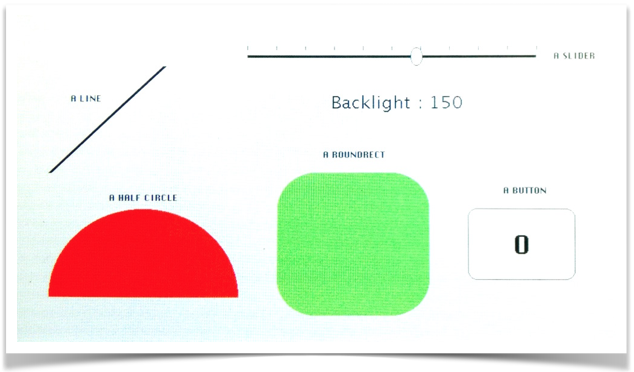
\includegraphics[width=6in]{AWFig1.png} 
   \caption{The AW\_doc\_example }
   \label{fig:1 }
\end{figure}


~\\Here is the complete listing : 

\begin{lstlisting}[language=Arduino]
//--- Project : ArduinoWidgets library
//--- Authors : Pierre Molinaro & Jean-Luc Bechennec
//--- Description : ArduinoWidgets library multiple views example 

#include <ArduinoWidgets.h>
#include <UTFT.h>

//--- This part is hardware dependent :
//--- Teensy 3.6 + LCD 7" with Touch, SSD1963 controler, resolution 800x480
//--- LCD type (see /Applications/Arduino.app/Contents/Java/hardware/teensy/avr/libraries/UTFT/UTFT.h)

static const byte RS    = 23 ;
static const byte WR    = 22 ;
static const byte CS    = 15 ;
static const byte RESET = 33 ;

//--- Warning D33 of Teensy 3.1: 
//--- https://forum.pjrc.com/threads/24823-Teensy-3-1-Tying-Pin-33-(pta4)-low-freezes-teensy

//--- Do not change 'myGLCD' name; it is declared as extern in AWContext.cpp

UTFT myGLCD (SSD1963_800ALT, RS, WR, CS, RESET) ;

static const byte T_CLK  = 11 ;
static const byte T_CS   = 12 ;
static const byte T_DIN  = 25 ;
static const byte T_DOUT = 24 ;
static const byte T_IRQ  = 28 ;

static const byte BACKLIGHT = 9 ;

//--- Do not change 'myTouch' name; it is declared as extern in AWContext.cpp
AWTouch myTouch (T_CLK, T_CS, T_DIN, T_DOUT, T_IRQ) ;

//--- end of hardware dependent part

////////////////////////////////////////////////////////////////
//--- Definitions of behaviours of existing Views in the library
////////////////////////////////////////////////////////////////

/////////////////////////// BUTTON /////////////////////////////

//--- button related global variable
int buttonValue = 0 ;

//--- button action
void bigButtonAction (AWView * inSender)
{
  AWPushButton * sendingButton = (AWPushButton *) inSender ;
  buttonValue ++ ;
  sendingButton->setTitle (String(buttonValue)) ;
  digitalWrite (LED_BUILTIN, !digitalRead(LED_BUILTIN));
}

//////////////// SLIDER //////////////////////

//--- Slider global variables
AWSlider *backlightSlider;
AWLabel * label1;   // constant label
AWLabel * label2;   // variable label
//--- Slider action
void sliderAction (AWView * inSender)
{
  AWSlider * sendingSlider = (AWSlider *) inSender ;
  AWInt pos = sendingSlider->knobPosition ();
  if (sendingSlider == backlightSlider) {
    analogWrite (BACKLIGHT, pos);
    label2->setTitle(pos);
  }
}

//////////////////////////////////////
//--- Definitions of new View classes 
//////////////////////////////////////

/////////////// ROUND CORNERS RECTANGLE ///////////////

class CustomView1 : public AWView
{
  CustomView1 (const AWRect & inViewFrame);
  virtual void drawInRegion (const AWRegion & inRegion) const;
};
CustomView1::CustomView1 (const AWRect & inViewFrame) :
AWView(inViewFrame, 
  AWColor ()),                  // let the corners opaque, outside the drawing region
  Color2 (AWColor::green ()) 
  { }
void CustomView1::drawInRegion (const AWRegion & inRegion) const
{
  AWRect viewFrame = absoluteFrame () ;
  AWContext::setColor (Color2) ;
  viewFrame.fillRoundRectInRegion (AWInt (50), inRegion) ; // radius of corners is 50
}
//--- Global variable ROUNDRECT
CustomView1 * roundRectView ;

///////////// CLIPPING VIEW : A HALF CIRCLE /////////////

class ClippingView : public AWView
{
  ClippingView (const AWRect & inViewFrame);
  virtual void drawInRegion (const AWRegion & inRegion) const;
};
ClippingView::ClippingView (const AWRect & inViewFrame) :
AWView(inViewFrame, 
  AWColor ())           // outside the drawing region is opaque 
  { }
void ClippingView::drawInRegion (const AWRegion & inRegion) const
{
  AWRegion drawingRegion = inRegion ;
  AWRect viewFrame = absoluteFrame () ;
  AWRect clipRectangle = viewFrame ;
  clipRectangle.size.width /= 1 ;
  clipRectangle.size.height /= 2 ;    // the clip rectangle hide the low half of the circle
  drawingRegion -= clipRectangle ;
  AWContext::setColor (AWColor::red ());
  viewFrame.fillOvalInRegion (drawingRegion) ;
}
//--- Global variable CLIPPING VIEW
ClippingView * crossView ;


/////////////////////// SETUP //////////////////////////////

void setup() {
//--- This part is hardware dependent
//--- set up the backlight
  analogWrite (BACKLIGHT, 150);
  pinMode (LED_BUILTIN, OUTPUT);
  digitalWrite (LED_BUILTIN, HIGH);

  AWContext::begin (kOrientationLandscape,
                    800,      // Screen width
                    480,      // Screen height
                    true,     // true : X is flipped
                    false) ;  // false : Y is not flipped

//--- end of hardware dependent part

//--- create a button on screen
  AWPushButton * bigButton = new AWPushButton(AWRect (600, 100, 140, 100), String (buttonValue), AWFont (ChicagoDigit36)) ;
  bigButton->setAction (bigButtonAction) ; 
  addView (new AWLabel (AWPoint (625, 220), 100, kAWAlignmentCenter, "A BUTTON")) ;
  addView (bigButton) ; 

//--- create 2 labels, one constant and one that can be changed by the slider 
  label1 = new AWLabel(AWPoint ( 300, 340), AWInt (250), AWAlignment (kAWAlignmentRight), String ("Backlight : "), AWFont (Lucida_Grande24)) ;
  addView (label1) ;
  label2 = new AWLabel(AWPoint ( 550, 340), AWInt (100), AWAlignment (kAWAlignmentLeft), String ("150"), AWFont (Lucida_Grande24)) ;
  addView (label2) ;

//--- create the slider with its label
  backlightSlider = new AWSlider (AWPoint (300,400), 400, kHorizontal, true) ;
  backlightSlider->setMaxKnobPosition (255);
  backlightSlider->setKnobPosition (150);
  backlightSlider->setAction (sliderAction);
  addView (new AWLabel (AWPoint (690, 410), 100, kAWAlignmentCenter, "A SLIDER")) ;
  addView (backlightSlider) ;

//--- create a black line of 5 pixel of thickness
  AWPoint lineOrigin ;
  lineOrigin.x = 50 ;
  lineOrigin.y = 250 ;
  AWPoint lineEnd;
  lineEnd.x = 200 ;
  lineEnd.y = 400 ;
  for (int i=0 ; i < 5 ; i++) {
    addView (new AWLine (lineOrigin, lineEnd)) ;
    lineOrigin.x++;
    lineEnd.x++;
  }
  addView (new AWLabel (AWPoint (50, 350), 100, kAWAlignmentCenter, "A LINE")) ;

//--- create the roundRect
  roundRectView = new CustomView1(AWRect (350, 50, 200, 200)) ;
  addView (roundRectView) ;   
  addView (new AWLabel (AWPoint (400, 270), 100, kAWAlignmentCenter, "A ROUNDRECT")) ;

//--- create the clipping view (half-circle)
  crossView = new ClippingView(AWRect (50, -50, 250, 250)) ;
  addView (crossView) ;
  addView (new AWLabel (AWPoint (100, 210), 150, kAWAlignmentCenter, "A HALF CIRCLE")) ;
  
  }

///////////////////////////// LOOP /////////////////

void loop() {
  AWContext::handleTouchAndDisplay () ;
}
\end{lstlisting}

~\\ To run this programme, it is recommended to open de sketch in the example folder of the ArduinoWidgets library, because a small file must be present in the same folder as the sketch. Its name must be "touch-calibration-values.h" and it must contain :

\begin{lstlisting}[language=Arduinonl]
#include "touch-calibration-values.h"

const float xA =  310.0 ; // 571.0 ;
const float yA =  116.0 ; // 963.0 ;

const float xB = 3811.0 ; // 488.0 ;
const float yB =  113.0 ; // 3001.0 ;

const float xC = 3814.0 ; // 3526.0 ;
const float yC = 3936.0 ; // 3349.0 ;

const float xD =  362.0 ; // 3519.0 ;
const float yD = 3938.0 ; // 698.0 ;
\end{lstlisting}

~\\ This .cpp file contain the values of the calibration of your screen.
If this file is not present in the sketch folder, a compilation error will occur

\begin{lstlisting}[language=Arduinonl]
.../AWContext.cpp:617: undefined reference to `yA'
.../AWContext.cpp:642: undefined reference to `xA'
.../AWContext.cpp:643: undefined reference to `yB'
.../AWContext.cpp:643: undefined reference to `yC'
.../AWContext.cpp:643: undefined reference to `xB'
.../AWContext.cpp:643: undefined reference to `yD'
.../AWContext.cpp:643: undefined reference to `xC'
.../AWContext.cpp:634: undefined reference to `xD'
\end{lstlisting}

~\\ Go to the section "Calibration" to know how to calibrate your touch screen.

%%%%%%%%%%%%%%%%%%%%%%%%%%%%%%%%%%%
\newpage
\section{A quick overview of the AW\_doc\_example}

~\\This section is not an in depth description on how to use each object of the library but just a global introduction to how to build a program which use the ArduinoWidgets library. A detailed description of the library is given farther in this document.

~\\ The program is divided in five parts :
\begin{itemize}
  \item The first part is to include the necessary libraries.
  \item The second part is the necessary adaptation to your hardware.
  \item The third part is the declaration of new graphic objets, the specific behaviors of existing objects of the library and the declarations of variables.
  \item The fourth part is the setup() function
  \item The fifth part is the loop() function.
\end{itemize}

~\\The first step is to import the two necessary libraries \texttt{ArduinoWidgets} and \texttt{UTFT} .
\begin{lstlisting}[language=Arduinonl]
#include <ArduinoWidgets.h>
#include <UTFT.h>
\end{lstlisting}

~\\Before using your specific Touch LCD display, please read the following documents which are located inside the UTFT/documentation folder :

\begin{itemize}
\item  "UTFT\_Requirements.pdf" for describing the pins which are used to connect your micro-controller to your LCD 
 \item "UTFT\_Supported\_display\_modules\_\&\_controllers.pdf" for finding the right declaration of the controller which is used in your screen 
\end{itemize}

~\\Then adapt the hardware dependent part 1 in the listing to your specific hardware :
 
 \begin{lstlisting}[language=Arduinonl]
//--- This part is hardware dependent, such as here :
//--- Teensy 3.6 + LCD 7" with Touch, 
//--- SSD1963 controler, resolution 800x480

static const byte RS    = 23 ;
static const byte WR    = 22 ;
static const byte CS    = 15 ;
static const byte RESET = 33 ;

//--- Do not change 'myGLCD' name; 
//--- it is declared as extern in AWContext.cpp

UTFT myGLCD (SSD1963_800ALT, RS, WR, CS, RESET) ;

static const byte T_CLK  = 11 ;
static const byte T_CS   = 12 ;
static const byte T_DIN  = 25 ;
static const byte T_DOUT = 24 ;
static const byte T_IRQ  = 28 ;

static const byte BACKLIGHT = 9 ;

//--- Do not change 'myTouch' name; 
//--- it is declared as extern in AWContext.cpp

AWTouch myTouch (T_CLK, T_CS, T_DIN, T_DOUT, T_IRQ) ;

//--- end of hardware dependent part  
\end{lstlisting}

~\\ At this stage, dont forget to add the file "touch-calibration-values.h" which must be present in the same folder as the sketch (see the end of section 3).
  
~\\Then add the specific customizations and creations of the objets to display on the screen, with the desired interactivity :

\begin{itemize}
\item  a value to display inside a button and an action when clicking in the button, which increment the button's value; 
 \item some variables and an action to be attached to a slider which control the brightness of the backlight of the screen;
 \item a new AWView object to display a rectangle with round corners;
 \item a new AWView object to display a half circle which is the combination of a full circle with a clipping rectangle.
\end{itemize}

~\\Then the \texttt{setup()} function initialize the backlight of the LCD to the value 150 (the maximum is 255). 
~\\Then it initialize the LCD with the proper parameters (orientation, size, X and Y directions). Please note that the origine (0,0) of the screen is in the lower-left corner, exactly as in a Cartesian coordinate system.
~\\The objects are then created :

\begin{itemize}
\item  the button and its label; 
 \item two labels, one of which is associated to the action of the slider;
 \item the slider;
 \item a black line;
 \item the roundRect;
 \item the half circle;
\end{itemize}


\begin{lstlisting}[language=Arduinonl]
void setup() {
//--- This part is hardware dependent
//--- set up the backlight
  analogWrite (BACKLIGHT, 150);
  pinMode (LED_BUILTIN, OUTPUT);
  digitalWrite (LED_BUILTIN, HIGH);

  AWContext::begin (kOrientationLandscape,
                    800,      // Screen width
                    480,      // Screen height
                    true,     // true : X is flipped
                    false) ;  // false : Y is not flipped

//--- end of hardware dependent part

//--- create a button on screen
  AWPushButton * bigButton = new AWPushButton(AWRect (600, 100, 140, 100), String (buttonValue), AWFont (ChicagoDigit36)) ;
  bigButton->setAction (bigButtonAction) ; 
  addView (new AWLabel (AWPoint (625, 220), 100, kAWAlignmentCenter, "A BUTTON")) ;
  addView (bigButton) ; 

//--- create 2 labels, one constant and one that can be changed by the slider 
  label1 = new AWLabel(AWPoint ( 300, 340), AWInt (250), AWAlignment (kAWAlignmentRight), String ("Backlight : "), AWFont (Lucida_Grande24)) ;
  addView (label1) ;
  label2 = new AWLabel(AWPoint ( 550, 340), AWInt (100), AWAlignment (kAWAlignmentLeft), String ("150"), AWFont (Lucida_Grande24)) ;
  addView (label2) ;

//--- create the slider with its label
  backlightSlider = new AWSlider (AWPoint (300,400), 400, kHorizontal, true) ;
  backlightSlider->setMaxKnobPosition (255);
  backlightSlider->setKnobPosition (150);
  backlightSlider->setAction (sliderAction);
  addView (new AWLabel (AWPoint (690, 410), 100, kAWAlignmentCenter, "A SLIDER")) ;
  addView (backlightSlider) ;

//--- create a black line of 5 pixel of thickness
  AWPoint lineOrigin ;
  lineOrigin.x = 50 ;
  lineOrigin.y = 250 ;
  AWPoint lineEnd;
  lineEnd.x = 200 ;
  lineEnd.y = 400 ;
  for (int i=0 ; i < 5 ; i++) {
    addView (new AWLine (lineOrigin, lineEnd)) ;
    lineOrigin.x++;
    lineEnd.x++;
  }
  addView (new AWLabel (AWPoint (50, 350), 100, kAWAlignmentCenter, "A LINE")) ;

//--- create the roundRect
  roundRectView = new CustomView1(AWRect (350, 50, 200, 200)) ;
  addView (roundRectView) ;   
  addView (new AWLabel (AWPoint (400, 270), 100, kAWAlignmentCenter, "A ROUNDRECT")) ;

//--- create the clipping view (half-circle)
  crossView = new ClippingView(AWRect (50, -50, 250, 250)) ;
  addView (crossView) ;
  addView (new AWLabel (AWPoint (100, 210), 150, kAWAlignmentCenter, "A HALF CIRCLE")) ;
  
  }
  \end{lstlisting}

~\\The \texttt{loop()} function of the sketch is very simple since it contain only one instruction which do everything : get events and call actions: \texttt{handleTouchAndDisplay()} \\
 
\begin{lstlisting}[language=Arduinonl]
void loop() {
  AWContext::handleTouchAndDisplay () ;
}  
\end{lstlisting}
  
%%%%%%%%%%%%%%%%%%%%%%%%%%%%%%%%%%%
\newpage
\subsection{How to use the code lines of the following sections of \texttt{ArduinoWidgets}}

~\\In the following sections of this document, there is three pieces of Arduino code that will not be repeated.\\
~\\The first one is :
\begin{lstlisting}[language=Arduinonl]
#include <ArduinoWidgets.h>
#include <UTFT.h>
//--- This part is hardware dependent, such as here :
//--- Teensy 3.6 + LCD 7" with Touch, 
//--- SSD1963 controler, resolution 800x480

static const byte RS    = 23 ;
static const byte WR    = 22 ;
static const byte CS    = 15 ;
static const byte RESET = 33 ;

//--- Do not change 'myGLCD' name; 
//--- it is declared as extern in AWContext.cpp

UTFT myGLCD (SSD1963_800ALT, RS, WR, CS, RESET) ;

static const byte T_CLK  = 11 ;
static const byte T_CS   = 12 ;
static const byte T_DIN  = 25 ;
static const byte T_DOUT = 24 ;
static const byte T_IRQ  = 28 ;

static const byte BACKLIGHT = 9 ;

//--- Do not change 'myTouch' name; 
//--- it is declared as extern in AWContext.cpp

AWTouch myTouch (T_CLK, T_CS, T_DIN, T_DOUT, T_IRQ) ;

//--- end of hardware dependent part 

//--- add here you constants, classes, functions, variables, ...
\end{lstlisting}

~\\The second one is  the setup() :
\begin{lstlisting}[language=Arduinonl]
void setup() {
//--- This part is hardware dependent
//--- set up the backlight
  analogWrite (BACKLIGHT, 150);
  pinMode (LED_BUILTIN, OUTPUT);
  digitalWrite (LED_BUILTIN, HIGH);

  AWContext::begin (kOrientationLandscape,
                    800,      // Screen width
                    480,      // Screen height
                    true,     // true : X is flipped
                    false) ;  // false : Y is not flipped

//--- end of hardware dependent part

//--- add here your lines of code for setup

} //--- end of setup
\end{lstlisting}

~\\The third par is the \texttt{loop()} function of the sketch.
 
\begin{lstlisting}[language=Arduinonl]
void loop() {
  AWContext::handleTouchAndDisplay () ;
}  
\end{lstlisting}
~\\You can create an Arduino sketch by inserting first the 3 parts above, then the lines of code found in the various examples below.
  
~\\If you want to test the examples which are described in this document, the best way is to use the "example" menu of the Arduino's IDE. But you can also assemble the lines of code of each subsection with the above parts to be adapted first to you specific hardware.
  
%%%%%%%%%%%%%%%%%%%%%%%%%%%%%%%%%%%
\newpage
\section{The fondation of \texttt{ArduinoWidgets}}

~\\The \texttt{ArduinoWidgets} library is objet oriented (C++). It is made of a collection of objets which can be expanded later in future versions.

~\\The consequence is the naming and the syntax to use in your Arduino program : 
\begin{itemize}
\item Objetcts are named "classes".
\item Each class embedd its own variables which are hidden to your sketch.
\item Functions are named "methods".
\end{itemize}

~\\To create an instance of a class AWClass :

\begin{lstlisting}[language=Arduinonl]
AWClass * myObject;	// myObject is a pointer in memory
myObject = new AWClass(parameters of the constructor);
\end{lstlisting}

~\\To call a method of myObject :

~\\ If MyObject is a pointer :

\begin{lstlisting}[language=Arduinonl]
myObject->method(parameters);
\end{lstlisting}

~\\ If MyObject is a not a pointer :

\begin{lstlisting}[language=Arduinonl]
myObject.method(parameters);
\end{lstlisting}


%%%%%%%%%%%%%%%%%%%%
\subsection{Context}

~\\ The Context is the entire Screen you are using. You must know about Context before seeing something on your screen and touch it. 
~\\ To create a context, just call the "begin" function of AWContext.
~\\ The class AWContext is defined by :

\begin{lstlisting}[language=Arduinonl]
typedef enum {kOrientationLandscape, kOrientationPortrait} tOrientation ;

class AWContext {
  static void begin (const tOrientation inOrientation,
  			const AWInt inScreenWidth,
				const AWInt inScreenHeight,
				const bool inHorizontalFlip,
				const bool inVerticalFlip) ;
\end{lstlisting}

~\\ This is what is written in the example sketch :

\begin{lstlisting}[language=Arduinonl]
 AWContext::begin (kOrientationLandscape,
                    800,      // Screen width
                    480,      // Screen height
                    true,     // true : X is flipped
                    false) ;  // false : Y is not flipped
\end{lstlisting}

~\\ The Context have a variety of properties and methods, such as :

\begin{itemize}
\item A screen rectangle : you can get ths size on the screen rectangle
\begin{lstlisting}[language=Arduinonl]
//--- Screen rect
  static AWRect screenRect (void) ;
\end{lstlisting}

\item A color (backgroung color) : you can set or get the color of the screen and its opacity
\begin{lstlisting}[language=Arduinonl]
//--- Color
  static void setColor (const AWColor & inColor) ;
  static AWColor color (void) ;
  static bool colorIsOpaque (void) ;
\end{lstlisting}

\item A method for dealing with all events and actions of the touch screen and the display. This is the unique instruction in the loop() which work as a backgroud task in the examples.

\begin{lstlisting}[language=Arduinonl]
  static void handleTouchAndDisplay (void) ;
\end{lstlisting}

\item A calibrate method : 
\begin{lstlisting}[language=Arduinonl]
static void calibrateTouch (void) ;
\end{lstlisting}

\end{itemize}

%%%%%%%%%%%%%%%%%%%%%%
\subsection{The Views}

~\\ Every pieces of drawing on the screen are "Views".
~\\ A view is a rectangular section of the screen. It is responsible for handling all drawing and user-initiated events within its frame.

~\\ \texttt{ArduinoWidgets} provides the View class as an abstract view implementation that subclasses use as the basis for implementing custom display and user interaction.

~\\ In addition to drawing content and responding to user events, View instances act as containers for other views. By nesting views within other views, an application creates a hierarchy of views. This view hierarchy provides a clearly defined structure for how views draw relative to each other and pass messages from one view to another, up to the enclosing window, and on to the application for processing.

~\\ \texttt{ArduinoWidgets} provides several type of views for containing graphics, texts and controls which can send messages to its own view or to other views.

~\\ The root View is the screen.
~\\ Each View is placed in a parent View, the superview, in which it is a frame. This frame can be moved, resized, and rotated in the superview and the view's content moves with it.

~\\ The view is specified when a view instance is created programmatically using :

\begin{lstlisting}[language=Arduinonl]
//--- Constructor
  AWView (const AWRect & inRelativeFrame,
                   const AWColor & inBackColor) ;
 \end{lstlisting}

~\\ When it is necessary to know the frame rectangle of a view, the \texttt{absoluteFrame} method can return this absolute frame.

~\\ To translate a frame you can use the method \texttt{translateBy}. To change the frame size you can use \texttt{setSize}.
~\\ To specify or to get the backcolor of a view, you can use the methods \texttt{backColor} or \texttt{setBackColor}.

\begin{lstlisting}[language=Arduinonl]
//---------------- Frame
  inline AWRect absoluteFrame (void) const { return mAbsoluteFrame ; }

//---------------- Frame change
  void translateBy (const AWInt inDx, const AWInt inDy) ;
  void setSize (const AWSize & inNewSize) ;

//---------------- Background color
  inline AWColor backColor (void) const { return mBackColor ; }
  void setBackColor (const AWColor & inBackColor) ;
\end{lstlisting}

~\\ To add a new View on the screen, just call \texttt{addView} or \texttt{addCenteredView} :
\begin{lstlisting}[language=Arduinonl]
void addView (class AWView * inView) ;
void addCenteredView (class AWView * inView) ;
\end{lstlisting}

~\\\emph{What Is a View Hierarchy?}

~\\In addition to being responsible for drawing and handling user events, a view instance can act as a container, enclosing other view instances. Those views are linked together creating a view hierarchy. Unlike a class hierarchy, which defines the lineage of a class, the view hierarchy defines the layout of views relative to other views.

~\\The window instance maintains a reference to a single top-level view instance, call the content view. The content view acts as the root of the visible view hierarchy in a window. The view instances enclosed within a view are called subViews. The parent view that encloses a view is referred to as its superView. While a view instance can have multiple subViews, it can have only one superView. In order for a view and its subviews to be visible to the user, the view must be inserted into a window's view hierarchy.

~\\ A view is added to a parent view via the method \texttt{addSubView} or \texttt{addCenteredSubView}, in a hierarchical order :
\begin{lstlisting}[language=Arduinonl]
//---------------- Managing view hierarchy
  void addSubView (AWView * inView) ;         // if inView is non NULL, view is added in front of other subviews
  void addCenteredSubView (AWView * inView) ; // if inView is non NULL, view is added in front of other subviews
\end{lstlisting}

~\\To locate the superView use the method \texttt{superViev}. You can also remove a subView from a superView with \texttt{removeFromSuperView}.

\begin{lstlisting}[language=Arduinonl]
//---------------- Managing view hierarchy
  void addSubView (AWView * inView) ;         // if inView is non NULL, view is added in front of other subviews
  void addCenteredSubView (AWView * inView) ; // if inView is non NULL, view is added in front of other subviews
  void removeFromSuperView (void) ; // Does nothing if has no super view
  inline AWView * superView (void) { return mSuperView ; } // Returns NULL if has no super view
\end{lstlisting}

~\\\emph{View Tags}

~\\The View class defines methods that allow you to tag individual view objects with integer tags and to search the view hierarchy based on those tags. The receiver's subviews are searched depth-first, starting at the first subview returned by the receiver's subviews method.

The View method \texttt{tag} always returns –1. Subclasses can override this method to return a different value. It is common for a subclass to implement a \texttt{setTag} method that stores the tag value in an instance variable, allowing the tag to be set on an individual view basis. 

\begin{lstlisting}[language=Arduinonl]
//---------------- Tag
  inline void setTag (const int inTag) { mTag = inTag ; }
  inline int tag (void) const { return mTag ; }
\end{lstlisting}

~\\ \emph{User interactivity : sending and receiving Actions}

~\\A view or subview can be sensitive to touch actions of the user

\begin{lstlisting}[language=Arduinonl]
//---------------- Action
  void sendAction (void) ;
  inline AWAction action (void) const { return mAction ; }
  inline void setAction (AWAction inAction) { mAction = inAction ; }

//---------------- Touch
  virtual void touchDown (const AWPoint & inPoint) ;
  virtual void touchMove (const AWPoint & inPoint) ;
  virtual void touchUp (const AWPoint & inPoint) ;
\end{lstlisting}

~\\ \emph{Drawing and display views}

\begin{lstlisting}[language=Arduinonl]
//---------------- Display view
  void setNeedsDisplay (void) ;
  void setNeedsDisplayInRect (const AWRect & inRect) ;

//--- Draw method (to be overridden)
  virtual void drawInRegion (const AWRegion & inDrawRegion) const ;
\end{lstlisting}

~\\ A view can be opaque (drawable) or transparent (invalid or invisible).

\begin{lstlisting}[language=Arduinonl]
//--- Tell the view is opaque
  virtual bool isOpaque (void) const ;

//---------------- Visibility
  inline bool isVisible (void) const { return mIsVisible ; }
  void setVisibility (const bool inIsVisible) ;

//---------------- Handle "on screen" state
  public : inline bool isOnScreen (void) const { return mIsOnScreen ; }
\end{lstlisting}


~\\ More characteristics for managing Views, such as background color, opacity/transparency, resizing, translation, deletion, actions, touch, will be given in the corresponding detailed section.

~\\ There is an existing collection of ready to use Views which are :
\begin{itemize}
\item AWLine : display a line
\item AWLabel : display of text on a line.
\item AWPushButton : display a button
\item AWRectView : display a rectangle with or without round corners
\item AWSegmentedControl : display a radio button in a tab form
\item AWSlider : display a linear potentiometer with one cursor
\item AWDynamicSlider : display a linear potentiometer with one cursor
\item AWTabview : display tabs which are usefull for switching from one View to another. 
\item AWSwitch : display a check box. 
\item AWArrowPushButton : display a button with an arrow shape. 
\item AWKeyButton : display a key of keyboard 
\item AWKeyboardBackView : display an entire keyboard. 
\end{itemize}

~\\ You will be able to create and add your custom Views !

%%%%%%%%%%%%%%%%%%%%%%%%%%%%%%%%%%%%%%%%%%%%%%
\newpage
\subsection{Actions}

~\\ Some of the above Views can include one orseveral Actions
~\\ 
~\\ 

%%%%%%%%%%%%%%%%%%%%%%%%%%%%%%%%%%%
\newpage
\subsection{The coordinate plane}

~\\ A view is responsible for the drawing and event handling in a rectangular area of a window. In order to specify that rectangle of responsibility, you define its location as an origin point and size using a coordinate system.
~\\This section describes the coordinate system used by views, how a view's location and size is specified, and how the size of a view interacts with its content.

~\\ All information about location is given to \texttt{ArduinoWidgets} in terms of coordinates on a plane. The coordinate plane is a two-dimensional grid, as illustrated in Figure 2.

\begin{figure}[htbp]
   \centering
   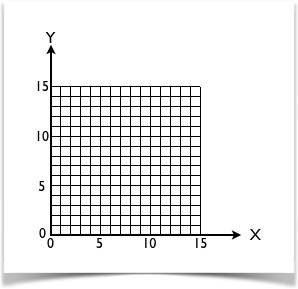
\includegraphics[scale=1]{AWFig2.png} 
   \caption{The coordinate plane}
   \label{fig:2 }
\end{figure}

~\\All grid coordinates are AWInt (in the range -32767 to 32767).

\begin{lstlisting}[language=Arduinonl]
typedef int16_t AWInt ;
\end{lstlisting}

~\\The origine of all coordinates is (0,0) and is located at the bottom left corner of the screen.
~\\Horizontal coordinates increase as you move from left to right, and vertical coordinates increase as you move from bottom to top. 

~\\ Each view use the same coordinate system as its mother view. 


%%%%%%%%%%%%%%%%%%%%
\newpage
\subsection{Points and Pixels}

~\\Each point is at the intersection of a horizontal grid line and a vertical grid line. 
~\\The coordinate origin (0,0) is in the lower-left corner of the screen. 

~\\You can store the coordinates of a point into an object AWPoint which contain 2 variables of type AWInt :

\begin{lstlisting}[language=Arduinonl]
// AWPoint :
  AWInt x ;
  AWInt y ;
\end{lstlisting}

~\\Figure 3 shows the relationship between points, grid lines, and pixels, the physical dots on the screen. 
A pixel is centered around a point. In other words, a point is at the center of a pixel.

\begin{figure}[htbp]
   \centering
   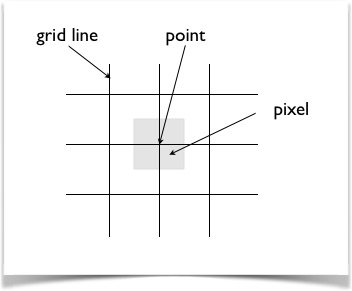
\includegraphics[scale=0.8]{AWFig3.png} 
   \caption{Points and Pixels}
   \label{fig:3 }
\end{figure}


~\\To create a AWPoint at coodinates X and Y, you call :
\begin{lstlisting}[language=Arduinonl]
AWPoint myPoint  ;
myPoint.x = X;
myPoint.y = Y;
\end{lstlisting}

~\\ The Point is not a View. The above myPoint is not drawed at this stage.

~\\ To compare two Points there is two special operators :
\begin{lstlisting}[language=Arduinonl]
//--- Equatable
  inline bool operator == (const AWPoint & inP) const { return (x == inP.x) && (y == inP.y) ; }
  inline bool operator != (const AWPoint & inP) const { return !(*this == inP) ; }
\end{lstlisting}

~\\ The Point class has the following methods :

\begin{lstlisting}[language=Arduinonl]
//--- Translation
  void translateBy (const AWInt inDx, const AWInt inDy) { x += inDx ; y += inDy ; }
  void translateBy (AWPoint & inTranslation) { x += inTranslation.x ; y += inTranslation.y ; }

//--- Stroke line
  void strokeLineInRegion (const AWPoint & inPoint, const AWRegion & inDrawRegion) const ;

  static void strokeLineInRegion (const AWInt inP1X,
                                           const AWInt inP1Y,
                                           const AWInt inP2X,
                                           const AWInt inP2Y,
                                           const AWRegion & inDrawRegion) ;

//--- Draw Point
  void drawInRegion (const AWRegion & inDrawRegion) const ;
  static void drawPointInRegion (const AWInt inX, const AWInt inY, const AWRegion & inDrawRegion) ;
\end{lstlisting}

~\\ And a special drawing of circle (?? how to use it ??)

\begin{lstlisting}[language=Arduinonl]
//--- Frame circle
  void frameCircleInRegion (const AWInt inRadius,
               const AWRegion & inDrawRegion) const ;

  static void frameCircleInRegion (const AWInt inCenterX,
            const AWInt inCenterY,
            const AWInt inRadius,
            const AWRegion & inDrawRegion) ;

//--- Fill circle
  void fillCircleInRegion (const AWInt inRadius,
            const AWRegion & inDrawRegion) const ;

   static void fillCircleInRegion (const AWInt inCenterX,
             const AWInt inCenterY,
             const AWInt inRadius,
             const AWRegion & inDrawRegion) ;
\end{lstlisting}

%%%%%%%%%%%%%%%%%%%%%%%%%%%%%%%%%%%%%%%%%%%%%%
\newpage
\subsection{Colors}

~\\ A color is defined by 3 bytes (uint\_8) and a boolean. The 3 bytes define respectively the red, green and blue component and the boolean "IsOpaque" define if the color is opaque or transparent.
~\\ A set of 17 colors is predefined to simplify your programming.
~\\ You can set colors, test colors or get colors.

\begin{lstlisting}[language=Arduinonl]
class AWColor {
//--- Default constructor (clear color)
  inline AWColor (void) : mRed (0), mGreen (0), mBlue (0), mIsOpaque (false) {}

//--- Constructor (custom color)
  inline AWColor (const uint8_t inRed,
                           const uint8_t inGreen,
                           const uint8_t inBlue) :
  mRed (inRed),
  mGreen (inGreen),
  mBlue (inBlue),
  mIsOpaque (true) {
  }

//--- Colors
  inline static AWColor black (void) {
    return AWColor (0, 0, 0) ;
  }
  inline static AWColor gray (void) {
    return AWColor (128, 128, 128) ;
  }
  inline static AWColor darkGray (void) {
    return AWColor (64, 64, 64) ;
  }
  inline static AWColor lightGray (void) {
    return AWColor (192, 192, 192) ;
  } 
  inline static AWColor veryLightGray (void) {
    return AWColor (224, 224, 224) ;
  } 
  inline static AWColor red (void) {
    return AWColor (255, 0, 0) ;
  }
  inline static AWColor green (void) {
    return AWColor (0, 255, 0) ;
  }
  inline static AWColor blue (void) {
    return AWColor (0, 0, 255) ;
  }
  inline static AWColor white (void) {
    return AWColor (255, 255, 255) ;
  }
  inline static AWColor yellow (void) {
    return AWColor (255, 255, 0) ;
  }
  inline static AWColor orange (void) {
    return AWColor (255, 127, 0) ;
  }
  inline static AWColor brown (void) {
    return AWColor (153, 102, 51) ;
  }
  inline static AWColor cyan (void) {
    return AWColor (0, 255, 255) ;
  }
  inline static AWColor magenta (void) {
    return AWColor (255, 0, 255) ;
  }
  inline static AWColor purple (void) {
    return AWColor (127, 0, 127) ;
  }
  inline static AWColor deepSkyBlue (void) {
    return AWColor (0, 0xBF, 255) ;
  }
  inline static AWColor lightSkyBlue (void) {
    return AWColor (0x87, 0xCE, 0xFA) ;
  }

//--- Equatable
  bool operator == (const AWColor & inOtherColor) const ;
  inline bool operator != (const AWColor & inOtherColor) const {
    return !(*this == inOtherColor) ;
  }

//--- Accessors
  inline uint8_t redComponent (void) const { return mRed ; }
  inline uint8_t greenComponent (void) const { return mGreen ; }
  inline uint8_t blueComponent (void) const { return mBlue ; }
  inline bool isOpaque (void) const { return mIsOpaque ; }
} ;
\end{lstlisting}


~\\ 
~\\ 
~\\ 

%%%%%%%%%%%%%%%%%%%%%%%%%%%%%%%%%%%%%%%%%%%%%%
\newpage
\subsection{Fonts}

~\\ 
~\\ 
~\\ 


%%%%%%%%%%%%%%%%%%%%%%%%%%%%%%%%%%%%%%%%%%%%%%
\newpage
\section{The Views of \texttt{ArduinoWidgets}}

~\\ This section describe the View classes which are already present in the \texttt{ArduinoWidgets} library, that you can use very simply.
\subsection{Lines}

~\\ A line is defined by 2 AWPoints. 
~\\ To create and draw a new line "myLine" from Point1 (50,50) and Point2 (400,400):

\begin{lstlisting}[language=Arduinonl]
//--- Constructor
  AWLine (const AWPoint & inRelativePoint1,
                   const AWPoint & inRelativePoint2) ;
 \end{lstlisting}

~\\ This example display a line from 100,100 to 300,300

\begin{lstlisting}[language=Arduinonl]
AWLine * myLine;
  myLine = new AWLine (AWPoint(100,100), AWPoint(300,300)); 
  addView (myLine) ;
 \end{lstlisting}
~\\ Note that in this case you cannot use the origin and destination points for further operations because they are only arguments of the constructor of myLine.

\begin{figure}[htbp]
   \centering
   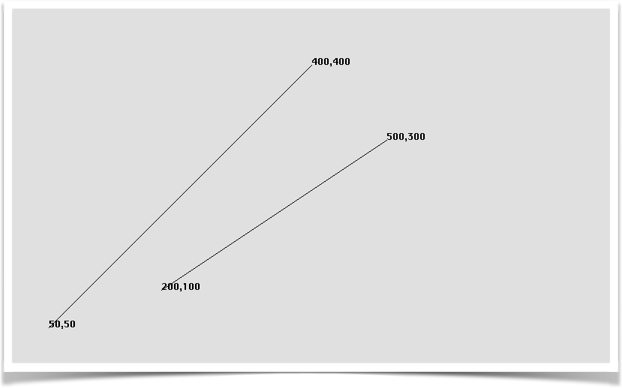
\includegraphics[scale=0.7]{AWFig4.png} 
   \caption{Points and Pixels}
   \label{fig:4 }
\end{figure}

  ~\\ This example display a line from AWPoint lineOrigin(50,50) to AWPoint lineEnd(400,400

\begin{lstlisting}[language=Arduinonl]
//--- create a black line
  AWPoint lineOrigin ;
  lineOrigin.x = 50 ;
  lineOrigin.y = 50 ;
  AWPoint lineEnd;
  lineEnd.x = 400 ;
  lineEnd.y = 400 ;
  AWLine * myLine1;
  myLine1 = new AWLine (lineOrigin, lineEnd); 
  addView (myLine1) ;
 \end{lstlisting}
~\\ Note that in this case you can use the lineOrigin and lineEnd points for further operations because they are declared outside the constructor of myLine1.
~\\ Note also that AWLine arguments are references (pointers) to AWPoints.

~\\ Note also that pixels are centered on points and, consequently, lines are centered on a grid line.

\begin{figure}[htbp]
   \centering
   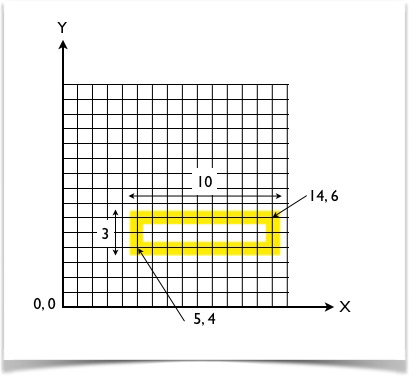
\includegraphics[scale=0.6]{AWFig5.png} 
   \caption{Lines and Pixels}
   \label{fig:5 }
\end{figure}

~\\ This figure explain why the dimensions of a line is one pixel more than the width or height used in the drawing method.

%%%%%%%%%%%%%%
\newpage
\subsection{Rectangles}

~\\ A Rectangle is defined by an origine AWPoint and an AWsize. The origine Point is the bottom-left corner :
\begin{lstlisting}[language=Arduinonl]
//--- Properties
  AWPoint origin ;
  AWSize size ;
  
// AWsize :
AWInt width ;
AWInt height ;

// AWRect :
myRect = new AWRect (AWPoint, AWSize);
myRect = new AWRect (X, Y, width, height);
\end{lstlisting}

~\\The coordinates of the bottom left corner are X = left, Y = bottom.
~\\ For example, you can create a new rectangle myRect of left-bottom corner X=350, Y=50, width W=200 and height H=200 like this :

\begin{lstlisting}[language=Arduinonl]
myRect = new AWRect (350, 50, 200, 200);
\end{lstlisting}

\begin{figure}[htbp]
   \centering
   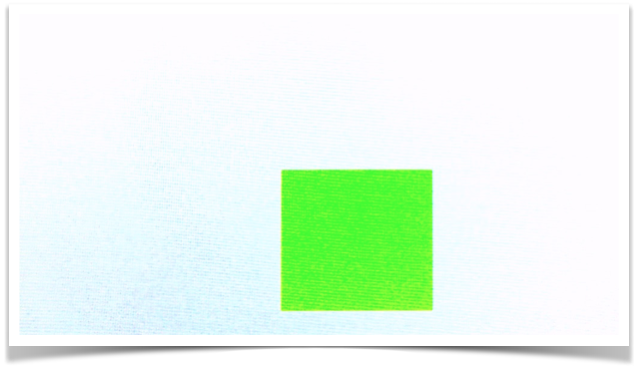
\includegraphics[scale=0.6]{AWFig6.png} 
   \caption{A Rectangle}
   \label{fig:6 }
\end{figure}

~\\ This rect have a bottom left corner origin of coordinates (350, 50).
~\\ The width (200) and height (200) are the number in pixels in the horizontal and vertical directions.
~\\ Consequently, the coordinate of the top right corner of this rectangle is (14, 6) :
\begin{itemize}
\item left = X = 350
\item bottom = Y = 50
\item right = X + W -1 = 350 + 200 -1 = 549
\item top = Y + H -1 = 50 + 200 -1 = 249
\end{itemize}


~\\ You also can create rectangle from various combinations of AWInt, AWPoint and AWSize. The constructors are :
\begin{lstlisting}[language=Arduinonl]
  //--- Constructors
  inline AWRect (const AWPoint inOrigin, const AWSize inSize) : 
  	origin (inOrigin), size (inSize) {}
  inline AWRect (const AWPoint inOrigin) : 
  	origin (inOrigin), size (AWSize (1, 1)) {} 
	// this is a single Point !
  inline AWRect (const AWInt inX, const AWInt inY, const AWInt inWidth, const AWInt inHeight) :
  	origin (AWPoint (inX, inY)), size (AWSize (inWidth, inHeight)) {}
  AWRect (const AWPoint & inP1, const AWPoint & inP2) ;
  static AWRect horizontalLine (const AWInt inX, const AWInt inY, const AWInt inWidth) ;
  static AWRect verticalLine (const AWInt inX, const AWInt inY, const AWInt inHeight) ;
\end{lstlisting}


~\\ You will see farther all the operations and transformations that you can do on AWRect such as :
\begin{itemize}
\item to be visible or invisible or empty (if W <=0 or H <=0)
\item a pixel is a rectangle with W = H =1
\item a horizontal line is a rectangle with W =1
\item a vertical line is a rectangle with H = 1
\item a 800x600 screen is a rectangle (0, 0, 800, 600)
\item find corners points
\item make intersection, inclusion or union of rectangles
\item find differences (the opposite of intersection) of rectangles
\item inset en translate rectangles
\item draw and fill rectangles, round-rectangles, and ovales
\end{itemize}

The AWRect methodes are :
\begin{lstlisting}[language=Arduinonl]
//--- Accessors
  inline bool isEmpty (void) const { return (size.width <= 0) || (size.height <= 0) ; }
  bool containsPoint (const AWPoint & inPoint) const ;
  AWPoint topRight (void) const ;
  AWPoint bottomRight (void) const ;
  AWPoint topLeft (void) const ;
  inline AWPoint bottomLeft (void) const { return origin ; }
  inline AWInt minX (void) const { return origin.x ; }
  inline AWInt maxX (void) const { return origin.x + size.width - 1 ; }
  inline AWInt minY (void) const { return origin.y ; }
  inline AWInt maxY (void) const { return origin.y + size.height - 1 ; }

//--- Intersection
  AWRect operator & (const AWRect & inOtherRect) const ;
  bool intersects (const AWRect & inOtherRect) const ;

//--- Inclusion
  bool includesRect (const AWRect & inOtherRect) const ;

//--- Union (Returns the smallest rectangle that completely encloses both receiver rect and inOtherRect)
  AWRect operator + (const AWRect & inOtherRect) const ;
  void operator += (const AWRect inOtherRect) ;

//--- Difference (Returns 4 rects, possibly empty)
  void differenceFrom (const AWRect & inRect,
                                AWRect & outR1,
                                AWRect & outR2,
                                AWRect & outR3,
                                AWRect & outR4) const ;

//--- Transforming rectangle
  void inset (const AWInt inDx, const AWInt inDy) ;
  void translateBy (const AWInt inDx, const AWInt inDy) ;

//--- Equatable
  bool operator == (const AWRect & inRect) const { return (origin == inRect.origin) && (size == inRect.size) ; }
  inline bool operator != (const AWRect & inRect) const { return ! (*this == inRect) ; }

//--- Drawing
  void fillRectInRegion (const AWRegion & inDrawRegion) const ;
  void frameRectInRegion (const AWRegion & inDrawRegion) const ;
  void fillRoundRectInRegion (const AWInt inRadius, const AWRegion & inDrawRegion) const ;
  void frameRoundRectInRegion (const AWInt inRadius, const AWRegion & inDrawRegion) const ;
  void fillOvalInRegion (const AWRegion & inDrawRegion) const ;
  void frameOvalInRegion (const AWRegion & inDrawRegion) const ;
\end{lstlisting}

~\\This example show how to display two rectangles : one without round corners and one with round corners :

~\\ First declare the new classes  RectangleView and RoundRectangleView, and create an instance of each class :

\begin{lstlisting}[language=Arduinonl]
/////////////// RECTANGLE ///////////////
class RectangleView : public AWView
{
  RectangleView (const AWRect & inViewFrame);
  virtual void drawInRegion (const AWRegion & inRegion) const;
};
RectangleView::RectangleView (const AWRect & inViewFrame) : // constructor
AWView(inViewFrame, 
  AWColor ()),             
  RectColor (AWColor::orange ()) 
  { }
void RectangleView::drawInRegion (const AWRegion & inRegion) const
{
  AWRect viewFrame = absoluteFrame () ;
  AWContext::setColor (RectColor) ;
  viewFrame.fillRectInRegion (inRegion) ;
}
//--- Global variable RectView
RectangleView * RectView ;

/////////////// ROUND CORNERS RECTANGLE ///////////////
class RoundRectangleView : public AWView
{
  RoundRectangleView (const AWRect & inViewFrame);
  virtual void drawInRegion (const AWRegion & inRegion) const;
};
RoundRectangleView::RoundRectangleView (const AWRect & inViewFrame) : // constructor
AWView(inViewFrame, 
  AWColor ()),             
  RectColor (AWColor::green ()) 
  { }
void RoundRectangleView::drawInRegion (const AWRegion & inRegion) const
{
  AWRect viewFrame = absoluteFrame () ;
  AWContext::setColor (RectColor) ;
  viewFrame.fillRoundRectInRegion (AWInt (50), inRegion) ;
}
//--- Global variable RoundRectView
RoundRectangleView * RoundRectView ;
\end{lstlisting}

~\\ Then draw the rectangles in the setup() :

\begin{lstlisting}[language=Arduinonl]
  //--- draw the Rectangle
  RectView = new RectangleView (AWRect (350, 50, 200, 300)) ;
  addView (RectView) ;   
  
  //--- draw the RoundRectangle
  RoundRectView = new RoundRectangleView (AWRect (80, 200, 250, 200)) ;
  addView (RoundRectView) ;   
\end{lstlisting}

\begin{figure}[htbp]
   \centering
   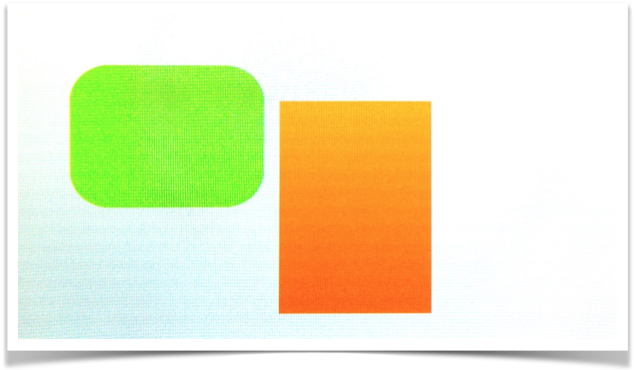
\includegraphics[scale=0.55]{AWFig7.png} 
   \caption{Two Rectangles}
   \label{fig:7}
\end{figure}


%%%%%%%%%%%%%%
\newpage
\subsection{Regions}

~\\ The minimum Region is a Rectangle or can be empty.
~\\ A Region is made of a combination of one or more separate and non-empty rectangles.
~\\ The role of a Region is to manage more or less complex geometric entities which are not limited to a Rectangle.

~\\ A Region is not a View and do not allow any drawing by itself, but it allow several operations.

\begin{lstlisting}[language=Arduinonl]
//--- Region from a rectangle (empty if rectangle is empty)
 AWRegion (const AWRect & inRect) ; 
 AWRegion(); // build an empty region
\end{lstlisting}
  
~\\ The purpose of regions is to limit drawing within the region. For example, if you want to draw a half circle on the screen, you can set the region to half the square that would enclose the whole circle, and then draw the whole circle. Only the half within the region will actually be drawn.

~\\ First declare the new classes  ClippingView :

\begin{lstlisting}[language=Arduinonl]
///////////// CLIPPING VIEW : A HALF CIRCLE /////////////
class ClippingView : public AWView
{
  ClippingView (const AWRect & inViewFrame);
  virtual void drawInRegion (const AWRegion & inRegion) const;
};
ClippingView::ClippingView (const AWRect & inViewFrame) :
  AWView(inViewFrame, 
  AWColor ())           // outside the drawing region is opaque 
  { }
void ClippingView::drawInRegion (const AWRegion & inRegion) const
{
  AWRegion drawingRegion = inRegion ;
  AWRect viewFrame = absoluteFrame () ;
  AWRect clipRectangle = viewFrame ;
  clipRectangle.size.width /= 1 ;
  clipRectangle.size.height /= 2 ;    // the clip rectangle hide the low half of the circle
  drawingRegion -= clipRectangle ;
  AWContext::setColor (AWColor::red ());
  viewFrame.fillOvalInRegion (drawingRegion) ;
}
//--- Global variable CLIPPING VIEW
ClippingView * crossView ;
\end{lstlisting}

~\\ Then draw the View in the setup() :
\begin{lstlisting}[language=Arduinonl]
//--- create the clipping view (half-circle
  crossView = new ClippingView(AWRect (300, 100, 250, 250)) ;
  addView (crossView) ;
\end{lstlisting}

~\\ A Region is defined by a rectangle which extends from the bottom left corner (300, 100) with size (250, 250). The circle is centered in this rectangle.
~\\ Then a clipRectangle is defined as a the bottom half of the Region's rectangle.
~\\ Then this bottom half is removed from the region.
~\\ Then the circle is drawn but only the top half is visible !

\begin{figure}[htbp]
   \centering
   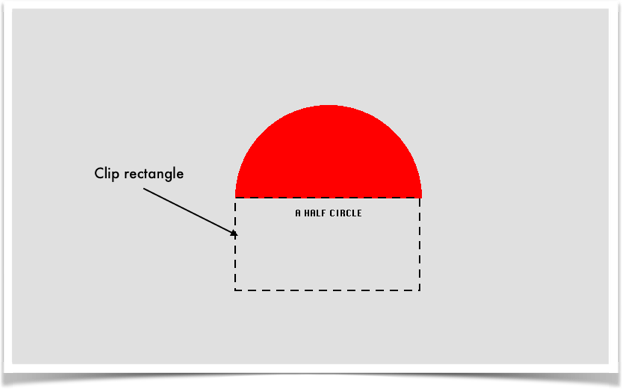
\includegraphics[scale=0.55]{AWFig8.png} 
   \caption{Region with clipping rectangle}
   \label{fig:8 }
\end{figure}


~\\ There is various operations on regions, wiich are defined in the methods of the class AWRegion:
\begin{lstlisting}[language=Arduinonl]
//--- release region, becomes empty
  void release (void) ;

//--- Accessors
  inline bool isEmpty (void) const 
     { return NULL == mPtr ; }
  AWInt rectCount (void) const ;
  AWRect rectAtIndex (const AWInt inIndex) const ;

//--- Difference from a rectangle
  void operator -= (const AWRect & inRect) ;

//--- Adding a rectangle
  void operator += (const AWRect & inRect) ;

//--- Intersection with a rectangle
  AWRegion operator & (const AWRect & inRect) const ;
  bool intersects (const AWRect & inOtherRect) const ;

//--- Intersection of regions
  AWRegion operator & (const AWRegion & inRect) const ;

//--- Enclosing rectangle
  AWRect enclosingRect (void) const ;

//--- Testing a point
  bool containsPoint (const AWPoint & inPoint) const ;
  bool containsPoint (
             const AWInt inX, 
             const AWInt inY
             ) const ;

//--- Handle copy
  AWRegion (const AWRegion & inRegion) ;
  AWRegion & operator = (const AWRegion & inRegion) ;
\end{lstlisting}


%%%%%%%%%%%%%%
\newpage
\subsection{Label and AutoLabel}

~\\ A Label is a string of text, "Title", that can be displayed anywhere on the screen (Context) or on a View or subView, or Region
~\\ You can choose a Point and a width to define where the Label is displayed (if the size of the Label is greater than the size, the Label will be clipped. You can choose the alignment of the text with this enum :

\begin{lstlisting}[language=Arduinonl]
typedef enum {
  kAWAlignmentLeft,
  kAWAlignmentCenter,
  kAWAlignmentRight
} AWAlignment ;
\end{lstlisting}

~\\ You can choose the style : the Font and size, the Color 
~\\ The Font and size is choosen from this list :
\begin{itemize}
\item ChicagoDigit36
\item ChicagoFLF12
\item ChicagoFLF24
\item Geneva10
\item Geneva12
\item Geneva9
\item LucidaGrande18
\item LucidaGrande24
\end{itemize}

~\\ You can choose the color from this list :
\begin{itemize}
\item black
\item gray
\item darkGray
\item lightGray
\item veryLightGray
\item red
\item green
\item blue
\item white
\item yellow
\item orange
\item brown
\item cyan
\item magenta
\item purple
\item deepSkyBlue
\item lightSkyBlue
\end{itemize}

~\\ or any other color according to the "Color" section 6.
~\\ Figure 9 show how it is simple to display a Label with these 2 lines of code in the setup():

\begin{lstlisting}[language=Arduinonl]
  addView (new AWLabel(AWPoint ( 300, 250), AWInt (250), AWAlignment (kAWAlignmentCenter), String ("ChicagoFLF24"), AWFont (ChicagoFLF24))) ;
\end{lstlisting}

~\\ or :

\begin{lstlisting}[language=Arduinonl]
  label = new AWLabel(AWPoint ( 300, 340), AWInt (150), AWAlignment (kAWAlignmentCenter), String ("Myabel : "), AWFont (Lucida_Grande24)) ;
  addView (label) ;
\end{lstlisting}

~\\ The constructor and methods of AWLabel are :

\begin{lstlisting}[language=Arduinonl]
class AWLabel : public AWView {
//---------- Constructor
  AWLabel (const AWPoint & inRelativeOrigin,
                    const AWInt inWidth,
                    const AWAlignment inAlignment,
                    const String & inTitle,
                    const AWFont & inFont = awkDefaultFont) ;

//----------- Draw
  virtual void drawInRegion (const AWRegion & inDrawRegion) const ;

//------------ Title
  void setTitle (const String & inTitle) ;
  String title (void) const { return mTitle; }

//------------ Text color
  void setTextColor (const AWColor & inColor) ;

//---------------- Font
  inline AWFont font (void) const { return mFont ; }

//------------ Alignment
  inline AWAlignment alignment (void) const { return mAlignment ; }
  void setAlignment (const AWAlignment inAlignment) ;
  };
\end{lstlisting}

\begin{figure}[htbp]
   \centering
   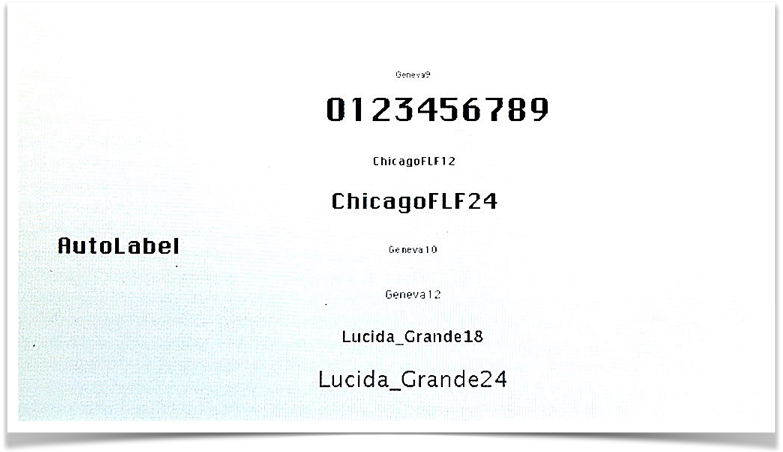
\includegraphics[scale=0.55]{AWFig9.png} 
   \caption{Labels and AutoLabel}
   \label{fig: 9}
\end{figure}


~\\ An AutoLabel is a simplified version of Label, without alignment and Width, which are calculated to match automatically the string :

\begin{lstlisting}[language=Arduinonl]
class AWAutoLabel : public AWView {
//--- Constructor
  AWAutoLabel (const AWPoint & inRelativeOrigin,
                        const String & inTitle,
                        const AWFont & inFont = awkDefaultFont) ;

//--- Draw
  virtual void drawInRegion (const AWRegion & inDrawRegion) const ;

//------------ Title
  void setTitle (const String & inTitle) ;

//------------ Text color
  void setTextColor (const AWColor & inColor) ;

//---------------- Font
  inline AWFont font (void) const { return mTextFont ; }
} ;
\end{lstlisting}

~\\ The code in the setup() for the Figure 9 is :

\begin{lstlisting}[language=Arduinonl]
  addView (new AWLabel(AWPoint ( 300, 50), AWInt (250), AWAlignment (kAWAlignmentCenter), String ("Lucida_Grande24"), AWFont (Lucida_Grande24))) ;
  addView (new AWLabel(AWPoint ( 300, 100), AWInt (250), AWAlignment (kAWAlignmentCenter), String ("Lucida_Grande18"), AWFont (Lucida_Grande18))) ;
  addView (new AWLabel(AWPoint ( 300, 150), AWInt (250), AWAlignment (kAWAlignmentCenter), String ("Geneva12"), AWFont (Geneva12))) ;
  addView (new AWLabel(AWPoint ( 300, 200), AWInt (250), AWAlignment (kAWAlignmentCenter), String ("Geneva10"), AWFont (Geneva10))) ;
  addView (new AWLabel(AWPoint ( 300, 250), AWInt (250), AWAlignment (kAWAlignmentCenter), String ("ChicagoFLF24"), AWFont (ChicagoFLF24))) ;
  addView (new AWLabel(AWPoint ( 300, 300), AWInt (250), AWAlignment (kAWAlignmentCenter), String ("ChicagoFLF12"), AWFont (ChicagoFLF12))) ;
  addView (new AWLabel(AWPoint ( 300, 350), AWInt (300), AWAlignment (kAWAlignmentCenter), String ("0123456789"), AWFont (ChicagoDigit36))) ;
  addView (new AWLabel(AWPoint ( 300, 400), AWInt (250), AWAlignment (kAWAlignmentCenter), String ("Geneva9"), AWFont (Geneva9))) ;

  addView (new AWAutoLabel(AWPoint ( 50, 200), String ("AutoLabel"), AWFont (ChicagoFLF24))) ;
\end{lstlisting}


%%%%%%%%%%%%%%
\newpage
\subsection{PushButton}

~\\ A PushButton is a View with an Action. The View is a roundRectangle with a Title inside.
~\\ We the user click inside the Button, an action is sent to a receiver.
~\\ The example below show a unique PushButton centered in the screen with a number inside. Each time you click in the button, the number inside the button is incremented.
~\\ The code for this example include a declaration before the setup() :

\begin{lstlisting}[language=Arduinonl]
//--- Current button value
int buttonValue = 0 ;

//--- button action
void bigButtonAction (AWView * inSender)
{
  AWPushButton * sendingButton = (AWPushButton *) inSender ;
  buttonValue ++ ;
  sendingButton->setTitle (String (buttonValue)) ;
}
\end{lstlisting}

~\\ and an initialization of the button in the setup() :
\begin{lstlisting}[language=Arduinonl]
 // create a big button centered on screen
  AWPushButton * bigButton = new AWPushButton(AWRect (0, 0, 300, 100), String (buttonValue), AWFont (ChicagoDigit36)) ;
  bigButton->setAction (bigButtonAction) ;
  addCenteredView (bigButton) ;
\end{lstlisting}

\begin{figure}[htbp]
   \centering
   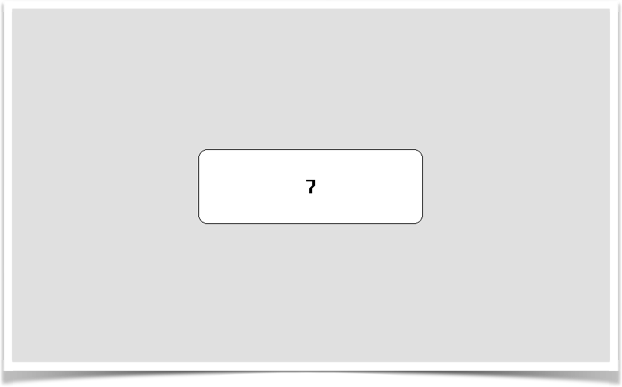
\includegraphics[scale=0.55]{AWFig10.png} 
   \caption{A PushButton}
   \label{fig: 10}
\end{figure}

~\\ The receiver of the PushButton is the Title of the button, but, in general, it can be any receiver inside any other object View.
~\\ The bigButtonAction function is activated each time there is a click in this button. It execute what you want to do.

~\\ The PushButton class contain the following constructor and methods

\begin{lstlisting}[language=Arduinonl]
class AWPushButton : public AWView {
  AWPushButton (const AWPoint & inRelativeBaselineOrigin,
                         const AWInt inWidth,
                         const String & inTitle,
                         const AWFont & inFont = awkDefaultFont) ;
  
  AWPushButton (const AWRect & inFrame,
                         const String & inTitle,
                         const AWFont & inFont = awkDefaultFont) ;
  
//------------ Title
  protected : String mTitle ;
  void setTitle (const String & inTitle) ;

//---------------- Font
  inline AWFont font (void) const { return mFont ; }

//--- Draw
  virtual void drawInRegion (const AWRegion & inDrawRegion) const ;

//--- Properties
  inline AWColor textColor (void) const { return mTextColor ; }
  void setTextColor (const AWColor inTextColor) { mTextColor = inTextColor ; }
  
  protected : AWInt mStringDisplayLength ;
  inline AWInt verticalMargin (void) const { return mVerticalMargin ; }

//--- Enabled state
  inline bool isEnabled (void) const { return mIsEnabled ; }
  void setEnabled (const bool inState) ;

//---------------- Hilite state
  inline bool isHilited (void) const { return mHiliteState ; }

//--- Tell the view is opaque or not
  virtual bool isOpaque (void) const ;

//--- Touch
  virtual void touchDown (const AWPoint & inPoint) ;
  virtual void touchMove (const AWPoint & inPoint) ;
  virtual void touchUp (const AWPoint & inPoint) ;
} ;
\end{lstlisting}


%%%%%%%%%%%%%%
\newpage
\subsection{SegmentedControl}

~\\ A SegmentedControl is 
~\\
~\\

\begin{figure}[htbp]
   \centering
   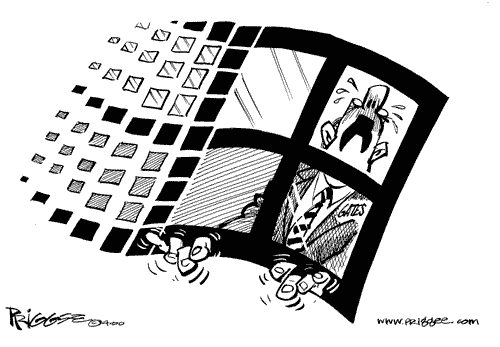
\includegraphics[scale=0.55]{AWFig.png} 
   \caption{Aie !! missing figure !}
   \label{fig:11}
\end{figure}

~\\

~\\ The SegmentedControl class contain the following constructor and methods

\begin{lstlisting}[language=Arduinonl]
typedef void (* AWSegmentedControlAction) (AWSegmentedControl * inSender, const AWInt inHilitedTabIndex) ;

class AWSegmentedControl : public AWView {
//--- Constructor
  AWSegmentedControl (const AWPoint & inRelativeBaselineOrigin,
                               const AWInt inWidth,
                               const AWFont & inFont = awkDefaultFont) ;

//--- Draw
  virtual void drawInRegion (const AWRegion & inDrawRegion) const ;

//--- Adding a Tab
  void addTab (const String & inTitle) ;

//--- Utilities
  AWRect tabTitleRectForIndex (const AWInt inIndex) const ;

//---------------- Font
  inline AWFont font (void) const { return mFont ; }

//--- Properties
  inline AWInt selectedTabIndex (void) const { return mSelectedTabIndex ; }
  void selectTabAtIndex (const AWInt inIndex) ;

//---------------- Segmented control action
// If segmented control action is NULL (by default), touch up changes selection and send action (defined in AWView)
// If not NULL, touch up does not change selection, and sends segmented control action
  inline AWSegmentedControlAction segmentedControlAction (void) const { return mSegmentedControlAction ; }
  inline void setSegmentedControlAction (const AWSegmentedControlAction inAction) {
    mSegmentedControlAction = inAction ;
  }

//---------------- Touch
  virtual void touchDown (const AWPoint & inPoint) ;
  virtual void touchMove (const AWPoint & inPoint) ;
  virtual void touchUp (const AWPoint & inPoint) ;

//---------------- Enabled state
  inline bool isEnabled (void) const { return mIsEnabled ; }
  void setEnabled (const bool inState) ;
} ;
\end{lstlisting}


%%%%%%%%%%%%%%
\newpage
\subsection{Slider}

~\\ A Slider is a complex View class which can control any entity by simply moving a cursor along a linear potentiometer
~\\ When the slider is moved (translated) an action is sent to a receiver with the value of the slider 
~\\ In this example, one slider control the brightness of the backlight of the screen, and the 3 other sliders control the color of a colorView (a simple rectangle).

\begin{figure}[htbp]
   \centering
   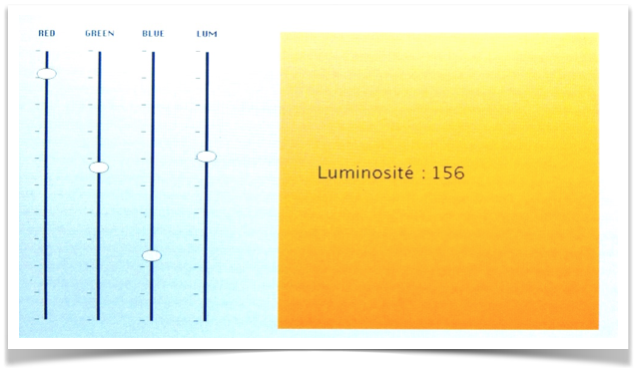
\includegraphics[scale=0.55]{AWFig12.png} 
   \caption{Four Sliders to control the brightness and the color of a Rectangle}
   \label{fig:12 }
\end{figure}

~\\ This exemple include a declaration part before the setup() :

\begin{lstlisting}[language=Arduinonl]
//--- Label
AWLabel * label1;
AWLabel * label2;

//--- Current color value
AWColor displayedColor = AWColor::white () ;

AWSlider *redSlider;
AWSlider *greenSlider;
AWSlider *blueSlider;
AWSlider *backlightSlider;
AWView *colorView;

//--- Slider action
void sliderAction (AWView * inSender)
{
  AWSlider * sendingSlider = (AWSlider *) inSender ;
  AWInt pos = sendingSlider->knobPosition ();
  if (sendingSlider == backlightSlider) {
    analogWrite (BACKLIGHT, pos);
    label2->setTitle(pos);
  }
  else {
    AWColor newColor(redSlider->knobPosition (), greenSlider->knobPosition (), blueSlider->knobPosition ());
    colorView->setBackColor (newColor) ;
  }
  \end{lstlisting}

~\\ and an initialization of the sliders and receivers in the setup() :

\begin{lstlisting}[language=Arduinonl]
 redSlider = new AWSlider (AWPoint (30,30), 400, kVertical, true) ;
  redSlider->setMaxKnobPosition (255);
  redSlider->setKnobPosition (255);
  redSlider->setAction (sliderAction);
  addView (redSlider) ;
  addView (new AWLabel (AWPoint (25, 440), 40, kAWAlignmentCenter, "RED")) ;
  
  greenSlider = new AWSlider (AWPoint (100,30), 400, kVertical, true) ;
  greenSlider->setMaxKnobPosition (255);
  greenSlider->setKnobPosition (255);
  greenSlider->setAction (sliderAction);
  addView (new AWLabel (AWPoint (95, 440), 40, kAWAlignmentCenter, "GREEN")) ;

  blueSlider = new AWSlider (AWPoint (170,30), 400, kVertical, true) ;
  blueSlider->setMaxKnobPosition (255);
  blueSlider->setKnobPosition (255);
  blueSlider->setAction (sliderAction);
  addView (new AWLabel (AWPoint (165, 440), 40, kAWAlignmentCenter, "BLUE")) ;

  backlightSlider = new AWSlider (AWPoint (240,30), 400, kVertical, true) ;
  backlightSlider->setMaxKnobPosition (255);
  backlightSlider->setKnobPosition (200);
  backlightSlider->setAction (sliderAction);
  addView (new AWLabel (AWPoint (235, 440), 40, kAWAlignmentCenter, "LUM")) ;

  addView (greenSlider) ;
  addView (blueSlider) ;
  addView (backlightSlider) ;
  colorView = new AWView (AWRect (350, 30, 420, 420), AWColor::white());
  addView (colorView) ;

  label1 = new AWLabel(AWPoint ( 400, 240), AWInt (150), AWAlignment (kAWAlignmentLeft), String ("Brightness : "), AWFont (Lucida\_Grande24)) ;
  addView (label1) ;
  label2 = new AWLabel(AWPoint ( 550, 240), AWInt (100), AWAlignment (kAWAlignmentLeft), String ("200"), AWFont (Lucida_Grande24)) ;
  addView (label2) ;
\end{lstlisting}

~\\ The Slider class contain the following constructor and methods

\begin{lstlisting}[language=Arduinonl]
const bool kHorizontal = false;
const bool kVertical = true;

class AWSlider : public AWView {
  AWSlider (const AWPoint & inOrigin,
                     const AWInt inSize,
                     const bool inOrientation,
                     const bool inHasRuler = true) ;

  //--- Draw
  virtual void drawInRegion ( const AWRegion & inDrawRegion ) const ;
   
  //--- Orientation
  bool orientation() const { return mOrientation ; }
  
  //--- Knob color
  protected : AWColor mKnobColor ;
  
  //--- Ruler display
  protected : void drawRulerInRegion ( const AWRegion & inDrawRegion ) const ;
  bool hasRuler() const { return mHasRuler ; }
  //--- Set the number of scales on the slider. Any value < 1 sets mHasRuler
  //--- to false so that no ruler is displayed
  void setHowManyScales ( const AWInt inHowManyScales ) ;
  
  //--- Position
  inline AWInt knobPosition (void) const { return mKnobPosition ; }
  void setKnobPosition ( AWInt inKnobPosition, const bool inRefresh = false ) ;
  inline AWInt maxKnobPosition (void) const { return mMaxKnobPosition ; }
  void setMaxKnobPosition ( AWInt inMaxKnobPosition ) ;
  protected : AWRect knobRect() const ;
  
  //--- Enabled state
  inline bool isEnabled (void) const { return mIsEnabled ; }
//  void setEnabled (const bool inState) ;
  
  //--- Tell the view is opaque or not
  virtual bool isOpaque (void) const ;
  
  //--- Touch
  virtual void touchDown (const AWPoint & inPoint) ;
  virtual void touchMove (const AWPoint & inPoint) ;
  virtual void touchUp (const AWPoint & inPoint) ;
  
} ;
\end{lstlisting}


%%%%%%%%%%%%%%
\newpage
\subsection{DynamicSlider}

~\\ A DynamicSlider is 
~\\
~\\

\begin{figure}[htbp]
   \centering
   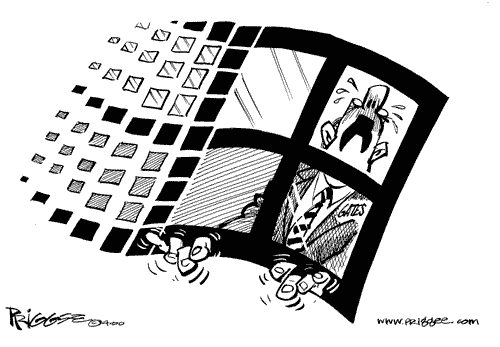
\includegraphics[scale=0.55]{AWFig.png} 
   \caption{Aie !! missing figure !}
   \label{fig:13}
\end{figure}

~\\

~\\ The DynamicSlider class contain the following constructor and methods

\begin{lstlisting}[language=Arduinonl]
class AWDynamicSlider : public AWSlider
{
  AWDynamicSlider ( const AWPoint & inOrigin,
                             const AWInt inSize,
                             const bool inOrientation,
                             const bool inHasRuler = true ) ;
  
  //--- Draw
  virtual void drawInRegion ( const AWRegion & inDrawRegion ) const ;
  
  //--- Position
  inline AWInt dynamicKnobPosition (void) const { return mDynKnobPosition ; }
  void setDynamicKnobPosition ( AWInt inKnobPosition ) ;
};
\end{lstlisting}


%%%%%%%%%%%%%%
\newpage
\subsection{TabView}

~\\ A TabView is 
~\\
~\\

\begin{figure}[htbp]
   \centering
   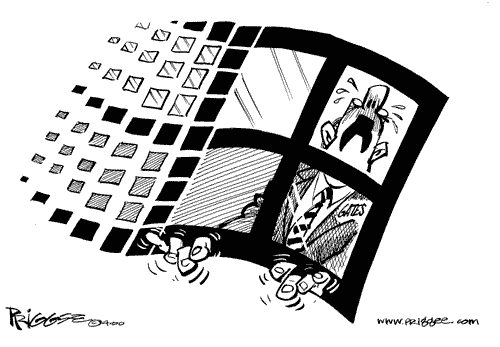
\includegraphics[scale=0.55]{AWFig.png} 
   \caption{Aie !! missing figure !}
   \label{fig:14 }
\end{figure}

~\\

~\\ The TabView class contain the following constructor and methods

\begin{lstlisting}[language=Arduinonl]
class AWTabView : public AWView {
//--- Constructor
  AWTabView (const AWRect & inRelativeFrame,
                      const AWFont & inFont = awkDefaultFont) ;

//--- Destructor
  virtual ~ AWTabView (void) ;

//--- Draw
  virtual void drawInRegion (const AWRegion & inDrawRegion) const ;

//--- Adding a Tab
  void addTab (const String & inTitle, AWView * inView) ;

//---------------- Font
  inline AWFont font (void) const { return mFont ; }

//--- Utilities
  AWInt titleHeight (void) const ;
  AWRect horizontalSeparator (void) const ;
  AWRect contentRectFromFrame (const AWRect & inFrame) const ;
  AWRect titleRect (void) const ;
  AWRect tabTitleRectForIndex (const AWInt inIndex) const ;

//--- Properties
  inline AWInt selectedTabIndex (void) const { return mSelectedTabIndex ; }
  void selectTabAtIndex (const AWInt inIndex) ;

//---------------- Badge
  void setBadgeAtIndex (const AWInt inIndex, const bool inDisplayBadge) ; // Does nothing if index if out of mList bounds
  bool hasBadgeAtIndex (const AWInt inIndex) const ; // return false if index if out of mList bounds
  AWRect badgeRect (const AWInt inItemIndex) const ;

//---------------- Touch
  virtual void touchDown (const AWPoint & inPoint) ;
  virtual void touchMove (const AWPoint & inPoint) ;
  virtual void touchUp (const AWPoint & inPoint) ;
} ;
\end{lstlisting}


%%%%%%%%%%%%%%
\newpage
\subsection{Switch}

~\\ A Switch is 
~\\
~\\

\begin{figure}[htbp]
   \centering
   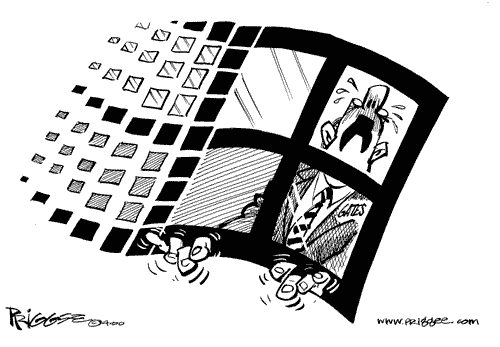
\includegraphics[scale=0.55]{AWFig.png} 
   \caption{Aie !! missing figure !}
   \label{fig:15 }
\end{figure}

~\\

~\\ The Switch class contain the following constructor and methods

\begin{lstlisting}[language=Arduinonl]
class AWSwitch : public AWView {
//--- Constructor
  AWSwitch (const AWPoint & inBaseLineRelativeOrigin,
                     const String & inTitle,
                     const AWFont & inFont = awkDefaultFont) ;

//--- Draw
  virtual void drawInRegion (const AWRegion & inDrawRegion) const ;

//---
  void setTitle (const String & inTitle) ;

  AWRect boxRect (void) const ;

//---------------- Font
  inline AWFont font (void) const { return mFont ; }

//------------- State
  inline bool checked (void) const { return mChecked ; }
  void setChecked (const bool inChecked) ;

//---------------- Hilite state
  protected : bool mHiliteState ; // false (by default): not hilited

//--- Enabled state
  inline bool isEnabled (void) const { return mIsEnabled ; }
  void setEnabled (const bool inState) ;

//---------------- Touch
  virtual void touchDown (const AWPoint & inPoint) ;
  virtual void touchMove (const AWPoint & inPoint) ;
  virtual void touchUp (const AWPoint & inPoint) ;
} ;
\end{lstlisting}


%%%%%%%%%%%%%%
\newpage
\subsection{ArrowPushButton}

~\\ An ArrowPushButton is 
~\\
~\\

\begin{figure}[htbp]
   \centering
   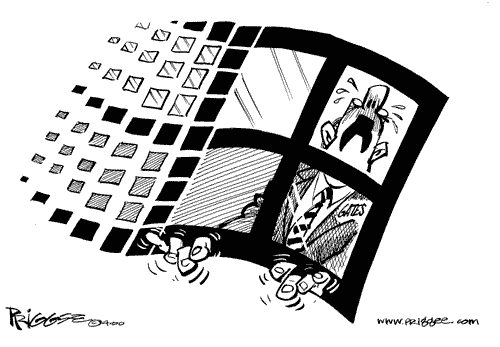
\includegraphics[scale=0.55]{AWFig.png} 
   \caption{Aie !! missing figure !}
   \label{fig:16 }
\end{figure}

~\\

~\\ The ArrowPushButton class contain the following constructor and methods

\begin{lstlisting}[language=Arduinonl]
enum { kUpArrow, kDownArrow, kRightArrow, kLeftArrow } ;

class AWArrowPushButton : public AWView
{
  public: AWArrowPushButton(const AWRect & inRelativeFrame,
                            const uint32_t inArrowDirection,
                            const AWColor & inArrowColor) ;

  //--- Arrow color
  private: uint32_t mArrowDirection ;
  //--- Arrow color
  private: AWColor mArrowColor ;
  public: AWColor arrowColor() const { return mArrowColor; } ;
  public: void setArrowColor(AWColor & inArrowColor) { mArrowColor = inArrowColor; } ;

  //--- Enabled state
  inline bool isEnabled (void) const { return mIsEnabled ; }
  void setEnabled (const bool inState) ;

  //--- On Off state management
  inline bool isOn() const { return mIsOn ; }
  inline void setIsOn (const bool inIsOn) { mIsOn = inIsOn ; }

  inline bool onOffState() const { return mOnOffState ; }
  inline void setOnOffState(const bool inOnOffState) { mOnOffState  = inOnOffState ; }

  //--- Draw
  virtual void drawInRegion (const AWRegion & inDrawRegion) const ;

  //--- Tell the view is opaque or not
  virtual bool isOpaque (void) const ;

  //--- Touch
  virtual void touchDown (const AWPoint & inPoint) ;
  virtual void touchMove (const AWPoint & inPoint) ;
  virtual void touchUp (const AWPoint & inPoint) ;
};
\end{lstlisting}


%%%%%%%%%%%%%%
\newpage
\subsection{KeyButton}

~\\ A KeyButton is 
~\\
~\\

\begin{figure}[htbp]
   \centering
   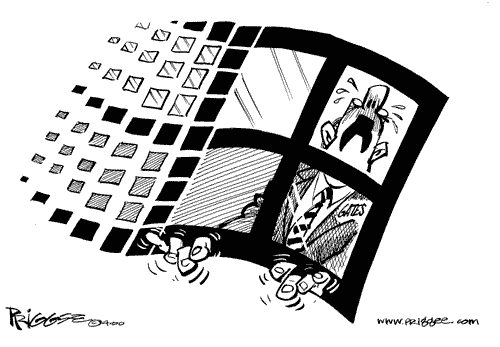
\includegraphics[scale=0.55]{AWFig.png} 
   \caption{Aie !! missing figure !}
   \label{fig:17}
\end{figure}

~\\

~\\ The KeyButton class contain the following constructor and methods

\begin{lstlisting}[language=Arduinonl]
class AWKeyButton : public AWView
{
  AWKeyButton (const AWRect & inFrame,
                        const AWColor & inBackColor) ;
  
  virtual void setShifted (const bool inShifted,
                                    const AWView * const inSender) ;

  //---------------- Hilite state
  inline bool isHilited (void) const { return mHiliteState; }
  
  //---------------- Drawing
  protected : void drawFrameAndBackgroundInRegion (const AWRegion & inDrawRegion) const ;
  virtual bool isOpaque (void) const ;

  //--- Touch
  virtual void touchDown (const AWPoint & inPoint) ;
  virtual void touchMove (const AWPoint & inPoint) ;
  virtual void touchUp (const AWPoint & inPoint) ;
};

class AWNormalKeyButton : public AWKeyButton
{
  AWNormalKeyButton (const AWRect & inFrame,
                              const char inText,
                              const char inShiftText) ;
  
  virtual void setShifted (const bool inShifted,
                                    const AWView * const inSender) ;
  
  char keyChar () const { return mCurrentKey ; }
  
  //--- Draw
  virtual void drawInRegion (const AWRegion & inDrawRegion) const ;
};

class AWReturnKeyButton : public AWKeyButton
{
  AWReturnKeyButton (const AWRect & inFrame) ;
  
  //--- Draw
  virtual void drawInRegion (const AWRegion & inDrawRegion) const ;
};

class AWBackspaceKeyButton : public AWKeyButton
{
  AWBackspaceKeyButton (const AWRect & inFrame) ;
  
  //--- Draw
  virtual void drawInRegion (const AWRegion & inDrawRegion) const ;
};

class AWShiftKeyButton : public AWKeyButton
{
  AWShiftKeyButton (const AWRect & inFrame, const bool inRightAlign) ;
  
  //---- Alignment of the arrow in the key
  virtual void setShifted (const bool inShifted,
                                    const AWView * const inSender) ;
  
  //--- Draw
  virtual void drawInRegion (const AWRegion & inDrawRegion) const ;
};

class AWLeftArrowKeyButton : public AWKeyButton
{
  AWLeftArrowKeyButton (const AWRect & inFrame) ;
  
  //--- Draw
  virtual void drawInRegion (const AWRegion & inDrawRegion) const ;
};

class AWRightArrowKeyButton : public AWKeyButton
{
  AWRightArrowKeyButton (const AWRect & inFrame) ;
  
  //--- Draw
  virtual void drawInRegion (const AWRegion & inDrawRegion) const ;
};
\end{lstlisting}


%%%%%%%%%%%%%%
\newpage
\subsection{Keyboard}

~\\ A Keyboard is 
~\\
~\\

\begin{figure}[htbp]
   \centering
   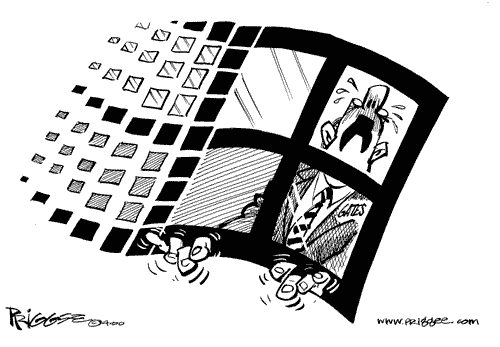
\includegraphics[scale=0.55]{AWFig.png} 
   \caption{Aie !! missing figure !}
   \label{fig:18 }
\end{figure}

~\\

~\\ The Keyboard class contain the following constructor and methods

\begin{lstlisting}[language=Arduinonl]
typedef void (*AWKeyboardCallback)(const String &inText, const int inTag);

void launchKeyboard (const String &inText,
                     const AWInt inMaxLength,
                     AWKeyboardCallback inCallback,
                     const int inTag = -1) ;
\end{lstlisting}


%%%%%%%%%%%%%%
\newpage
\section{The next steps of \texttt{ArduinoWidgets}}

~\\

~\\

~\\


%%%%%%%%%%%%%%%%%%%%%%%%%%%%%%%%%%%
\newpage
\section{The calibration of the Touch screen} 

~\\

~\\

~\\


%-----------------------------------------------------------------------------------------------------------------------*
%   F I N    D U    D O C U M E N T                                                                                     *
%-----------------------------------------------------------------------------------------------------------------------*

\end{document}
